\documentclass[10pt,a4paper]{article}
\usepackage[utf8]{inputenc}

\usepackage{amsmath}
\usepackage{amsfonts}
\usepackage{amssymb}
\usepackage{graphicx}
\usepackage{listings}
\usepackage[margin=1.0in]{geometry}
\usepackage{caption}
\usepackage{subcaption}
\usepackage{float}
\usepackage[utf8]{inputenc}
\usepackage{refstyle}


\lstset{numbers=left,
	title=\lstname,
	numberstyle=\tiny, 
	breaklines=true,
	tabsize=4,
	language=Python,
	morekeywords={with,super,as},,
	frame=single,
	basicstyle=\footnotesize\tt,
	commentstyle=\color{comment},
	keywordstyle=\color{keyword},
	stringstyle=\color{string},
	backgroundcolor=\color{background},
	showstringspaces=false,
	numbers=left,
	numbersep=5pt,
	literate=
		{æ}{{\ae}}1
		{å}{{\aa}}1
		{ø}{{\o}}1
		{Æ}{{\AE}}1
		{Å}{{\AA}}1
		{Ø}{{\O}}1
	}

\usepackage{bm}
\usepackage{hyperref}
\usepackage[usenames, dvipsnames]{color}

\begin{document}
\begin{center}
{\LARGE\bf
FYS4150\\

Project 4 - deadline November 19
}
\\
 
\includegraphics[scale=0.1]{uio.png}\\
Sander W. Losnedahl\\
University of Oslo, Autumn 2017
 
\end{center}

\begin{center}
{\Large\bf Abstract}
\end{center}

\noindent A c++ program have been developed to calculate various thermodynamic variables of a given lattice of objects using the popular two dimensional Ising model in the form if the Metropolis algorithm looped through Monte Carlo cycles. Other programs in MatLab have also been made to plot these variables against each other and do further calculations such as calculating the variance and critical temperature. The variables has shown to be very sensitive to temperature, rather than the initial configuration of the lattice. When the size of the lattice increases, the overall energy, magnetization, specific heat and susceptibility increase. However, the critical temperature, and therefore the phase shift, always happens when $T = 2.3$.

\newpage

\begin{center}
{\LARGE\bf Introduction}
\end{center}

\noindent This paper will look at the popular two dimensional Ising model which can determine phase transitions of a given lattice by first knowing the critical temperature. The model is however restricted in such a way that objects in the lattice can only have two values, in a so called binary system. In this paper, these two values represent upwards and downwards spin direction. Even though the model is restricted, it provides a good understanding of how phase transitions work.
\\
A simple 2 by 2 lattice will be studied first and is shown in \figref{22lattice}, where one can observe how the objects in the lattice interact with each other. The principle of the Ising model will later be extended to higher order lattices as well. Critical temperature and phase transitions will also be looked at near the end of the paper after necessary calculations have been made using the Metropolis algorithm.
\\
The codes and files used in this project can be found at \href{https://github.com/sanderwl/Assigment-4}{\textcolor{blue}{https://github.com/sanderwl/Assigment-4}}

\begin{figure}[H]
\centering
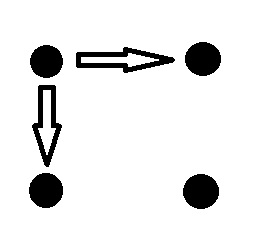
\includegraphics[width=0.5\textwidth]{22lattice}
\caption{A two by two lattice and how they interact using the Ising model}
\label{fig:22lattice}
\end{figure}

\newpage

\begin{center}
{\LARGE\bf Method}
\end{center}

\noindent To be able to start programming, one first needs to find the expressions for the partition function $Z$ with its corresponding energy values $E$, the mean magnetic moment $M$, the specific heat $C_V$ and the susceptibility $X$ as functions of the temperature $T$. All of this using the periodic boundary condition.
\\
The partition function $Z$ is giving by: 


$$
Z = \sum^{M}_{i = 1} e^{-\beta * E_i}
$$ 

\noindent where $\beta$ is the inverse temperature given by $\beta = \frac{1}{kT}$ where k is the Boltzmann constant and T is the temperature, so every expression containing $\beta$ is dependent on the temperature $T$. $E_i$ is the energy for different spin settings given by:

$$
E_i = -J\sum^{N}_{<kl>} s_ks_l
$$

\noindent where J is the coupling constant and N is the total number of spins. $s_k$ and $s_l$ are the spins of two neighbouring objects in a lattice. Since we are working 2x2 lattice, the total number of combinations are given by $2^4 = 16$, considering we are working with the Ising model where the spins can only be $-1$ or $1$.
\\
From \figref{22lattice} we see how the Ising model works on a 2x2 lattice and from this the energy is calculated. One can observe that energy is non-zero on lattices where all the objects have the same spin ($-8J$) and where the two diagonals have opposite spin from each other ($8J$). All other settings have zero energy. Knowing the energy values we can calculate the mean energy $<E>$ with our specific partition function:

$$
<E> = \frac{1}{Z}\sum^{M}_{i = 1} E_i e^{-\beta E_i}
$$
$$
 = \frac{1}{2e^{-8} + 2e^{8} + 12}\sum^{16}_{1} E_i e^{-\beta E_i}
$$
$$
 = \frac{16e^{-8}-16e^{8}}{2e^{-8} + 2e^{8} + 12} = -7.983928
$$

\noindent To find $Z$, one simply have to put the same energy values into the expression:

$$
Z = e^{-\beta * -8J} + e^{-\beta * -8J} + e^{-\beta * 8J} + e^{-\beta * 8J} + 12*e^0
$$
$$
Z = 2e^{-8J\beta} + 2e^{8J\beta} + 12
$$

\noindent The magnetization is given by:

$$
M = \sum^{N}_{j = 1} s_j
$$

\noindent Unlike in the energy case, the magnetization does not depend the lattice having the same spin or that the diagonals have opposite spin. The only case where the magnetization is zero in a 2x2 lattice is when half of the objects in the lattice opposite spins. Therefore we get the magnetization values:

$$
M_i = [4 + 2 + 2 + 2 + 2 + 0 + 0 + 0 + 0 + 0 + 0 + -2 + -2 + -2 + -2 + -4]
$$

\noindent To calculate the absolute value of the mean magnetic moment or mean magnetization we use the equation below with our calculated magnetic moment and energy values:

$$
|M| = \frac{1}{Z}\sum^{M}_{i}M_ie^{-\beta E_i}
$$
$$
 = \frac{1}{2e^{-8} + 2e^8 + 12}\sum^{16}_{1}M_ie^{-\beta E_i}
$$
$$
 = \frac{8e^{8} + 16}{2e^{-8} + 2e^8 + 12} = 3.994643
$$



\noindent To calculate the the specific heat, one only needs to know the total number of spins of the lattice. In the 2x2 lattice case the total number of spins is 4, and remember also that $\beta J = 1$ and $k = 1$. The specific heat is then:

$$
C_V = \frac{1}{kT^2}(<E^2> - <E>^2)
$$
$$
 = \frac{1}{kT^2}(\frac{128e^{-8} - 128e^8}{2e^{-8} + 2e^8 + 12} - (\frac{16e^{-8} - 16e^8}{2e^{-8} + 2e^8 + 12})^2)
$$
$$
 = 0.128329
$$

\noindent The term $<E^2> - <E>^2$ is also called the variance of the energy and is precisely calculated just as shown above. The same variance calculation can be applied to calculating the susceptibility, but the energy terms have to be substituted for mean magnetization.
Let's calculate the variance separate from the desired equation this time:

$$
\sigma_M^2 = <M^2>-<M>^2 = \frac{1}{Z}\sum^{M}_{i = 1}M_i^2 e^{-\beta E_i} - (\frac{1}{Z}\sum^{M}_{i = 1}M_i e^{-\beta E_i})^2
$$

$$
 = \frac{32}{2e^{-8} + 2e^8 + 12}(e^{8}+1) - (\frac{8e^8 + 16}{2e^{-8} + 2e^8 + 12})^2 = 0.016004
$$

\noindent Remember that the $\beta = 1$ in the 2x2 lattice case, so the susceptibility would be the same as the variance in that case. We would usually have to calculate the susceptibility with the following equation:

$$
X = \frac{1}{k_bT}(<M^2> - <M>^2) = \frac{1}{k_bT}\sigma_M^2 = 0.010853
$$

\noindent To compute the above values, a standard Metropolis algorithm were implemented. This algorithm takes an initial matrix and then decides to flip or not flip the current value at a random location in the matrix (lattice). The probability of when to flip or not is in this case given by the Boltzmann distribution $e^{-E_i / T}$. If the algorithm decides to flip, the computed energy at that position in the lattice is added to the total energy of the system. The same happens for the magnetization and initial values of the energy and magnetization is calculated beforehand. What initial matrix to use, that is a randomly generated matrix or a matrix with only positive spin, is determined by the user.\\

After the Metropolis algorithm is finished, the cumulative energy, squared cumulative energy, cumulative magnetization and squared cumulative magnetization is calculated which is needed to later calculate the mean energy, mean magnetization, specific heat and susceptibility. This algorithm is based on random events and so one needs to perform the algorithm many times before the results are stable. Therefore the whole Metropolis algorithm is looped inside what is called a Monte Carlo loop. When the number of Monte Carlo cycles are increased, the more stable the results will be. However, many cycles require a lot of processing power when the number of cycles gets to around $10^6$.
\\
To be able to run the program in a time efficient manner, one needs to parallellize the program, and this was done by using MPI with 8 processors. Using MPI made the processing time much smaller, but it still took a long time for large lattice sizes. The parallellized c++ program is found on GitHub, separate from the main program.
\\
Raw data were produced using c++ while plotting and further calculations were done using MatLab. Further calculations include finding the variance, the probability distribution and the critical temperature.  
\\
To calculate the critical temperature one have to use the following equation:

$$
T_c(L) - T_c(L=\infty) = aL^{-1/v}
$$

\noindent where $T_c$ is the critical temperature, L is the size of the lattice, $v = 1$ and a is a constant. $T_c(L)$ is known and we then get the following equations which can be solved numerically:

$$
T_c(L = \infty) = T_c(L) - aL^{-1}
$$

\noindent Again, $T_c$ and $L$ is known. The critical temperature values can also graphically found in the specific heat and susceptibility versus temperature plots for each lattice size. $1/L$ were then plotted against these critical temperatures and the least square rule was then used as the linear regression. By doing this, one would get a graph fitted towards the critical temperature points and where the graph hits the y-axis is the value of $T_c(L = \infty)$. Unfortunately, the plot showed $T_c$ to always be equal to $2.3$ due to too low resolution, meaning $T_c(L = \infty) = 2.3$ in this paper.

\newpage

\begin{center}
{\LARGE\bf Results}
\end{center}

\noindent The specific analytical value found in the method is compared to the numerical value calculated in c++ in the table below:

\begin{table} [H]
\caption{Analytical and numerical solutions when $T = 1.0$} \label{tab:table1}
\centerline{
\begin{tabular}{|c|c|c|c|}
\hline
Type & Analytical & Numerical & MC cycles needed\\
\hline
$<E>$ & -7.983928 & -7.98437 & $10^4$\\
\hline
$<M>$ & 3.994643 & 3.99483 & $10^4$\\
\hline
$C_V$ & 0.128329 & 0.124812 & $10^6$\\
\hline
$<X>$ & 0.016004 & 0.0153613 & $10^6$\\
\hline
\end{tabular}
}
\end{table}

\noindent To get good results for mean energy and mean magnetization took very few Monte Carlo cycles, only about $10^4$. Then the values would be off only by a factor of about $10^{-3}$. The susceptibility and the specific heat took more Monte Carlo cycles to get a precise and stable result. Correct results started showing around $10^{6}$. For $10^5$, both the specific heat and susceptibility gave varying results. 
\\
The values shown in Table \ref{tab:table1} are representing the entirety of the lattice. To transition from lattice wide values to single object values, one simply have to divide by the size of the lattice, $4$ in the above case, and multiply in the reverse case. The following results are for a 20 by 20 lattice:

\begin{figure}[H]
\centerline{
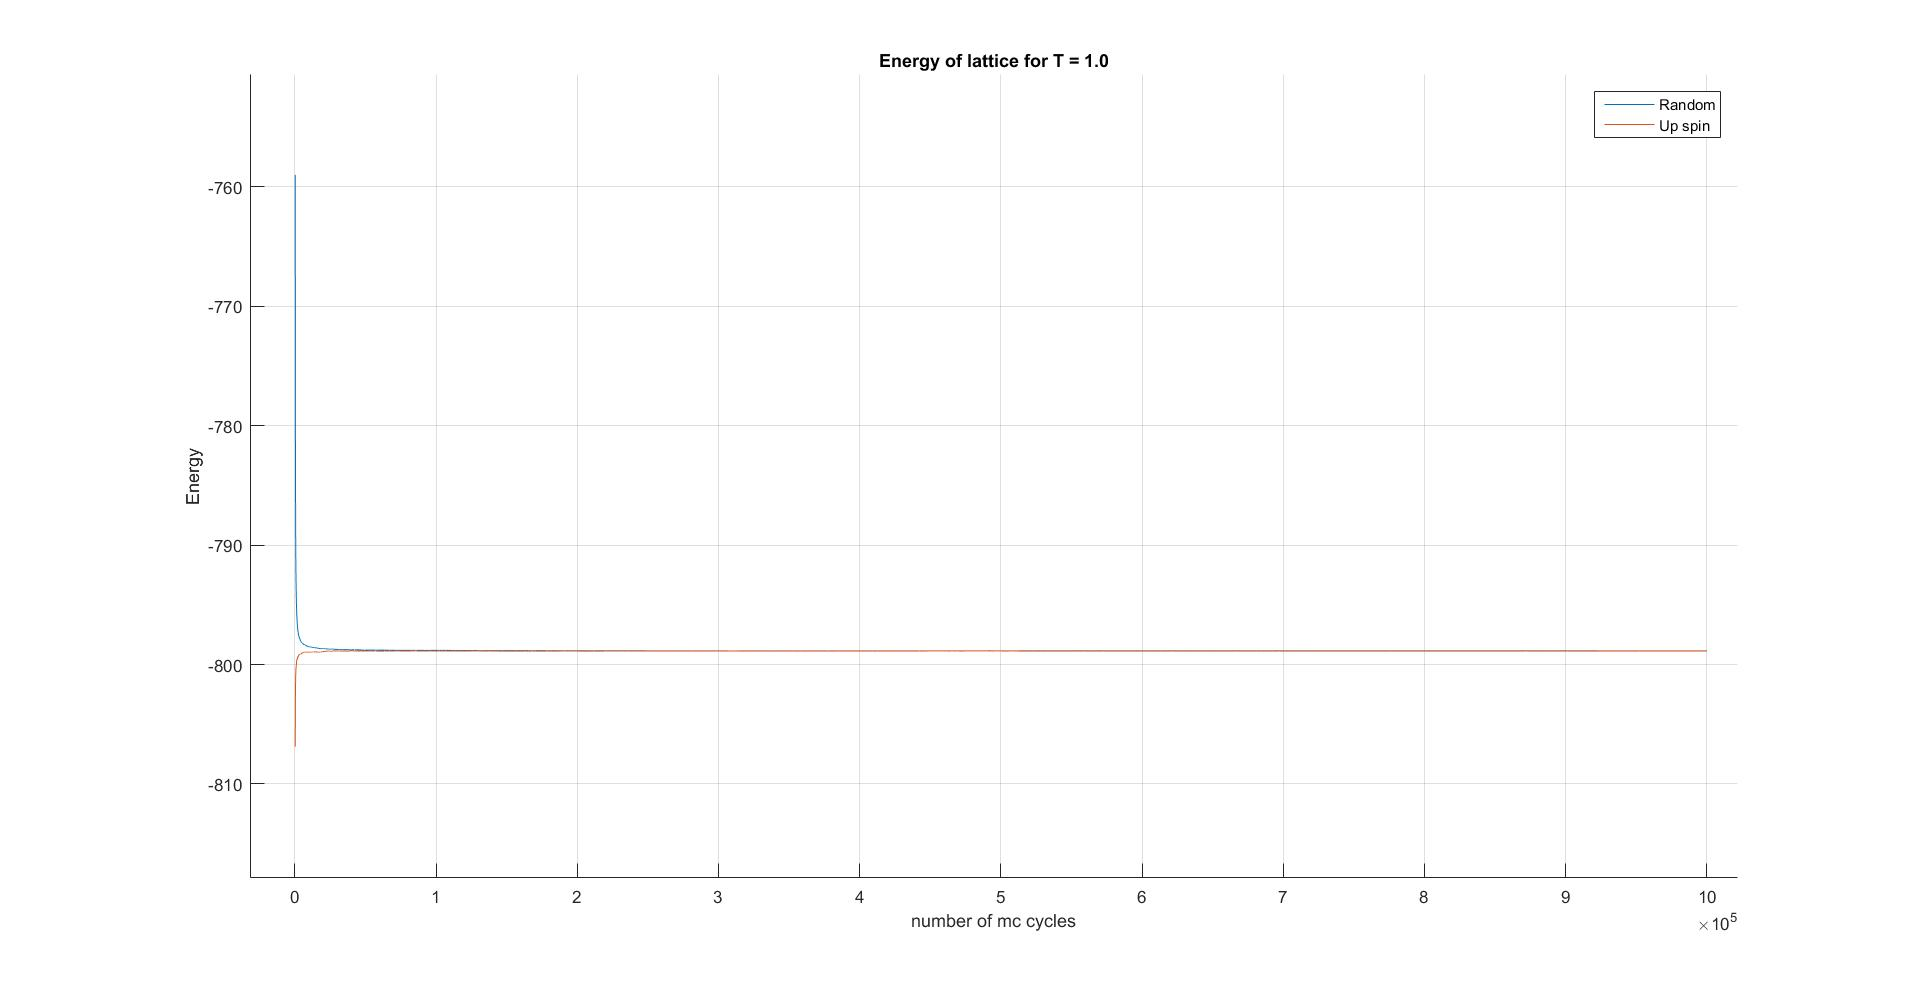
\includegraphics[width=0.7\textwidth]{energy1T}
}
\caption{Energy versus Monte Carlo cycles for T = 1.0}
\label{fig:energy1T}
\end{figure}

\begin{figure}[H]
\centerline{
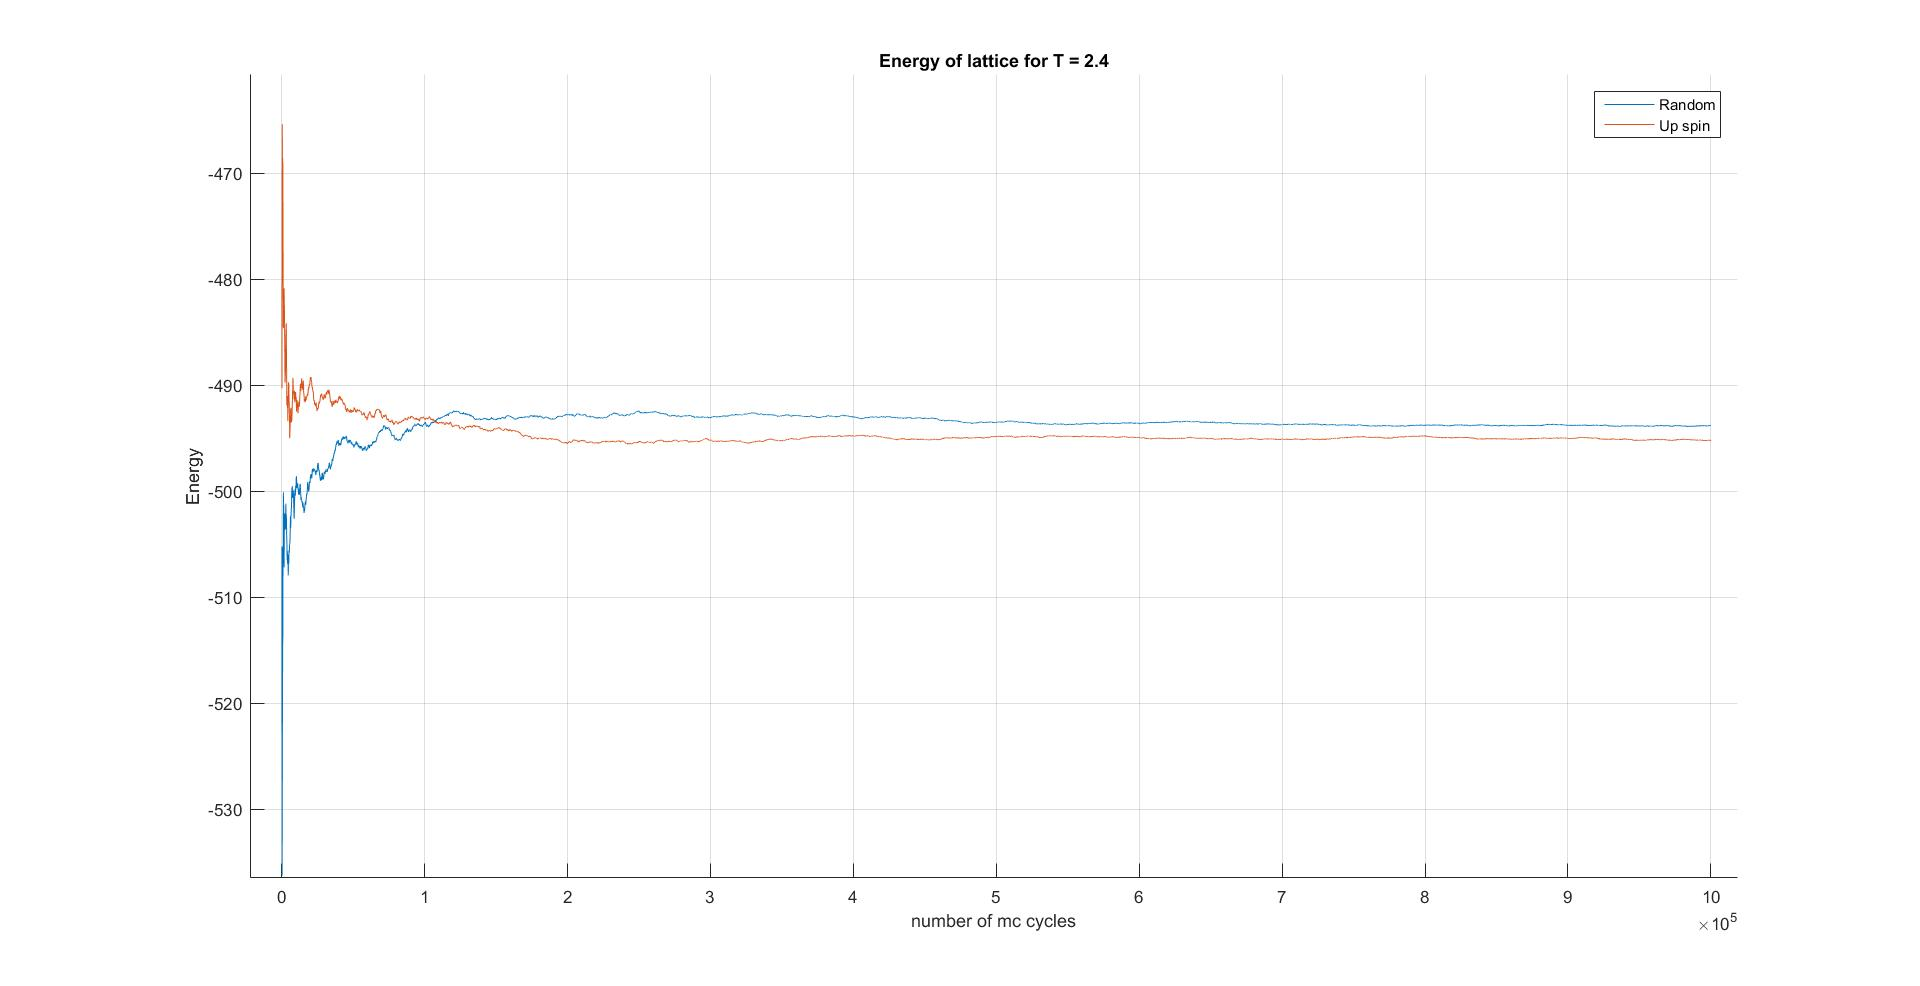
\includegraphics[width=0.7\textwidth]{energy24T}
}
\caption{Energy versus Monte Carlo cycles for T = 2.4}
\label{fig:energy24T}
\end{figure}

\begin{figure}[H]
\centerline{
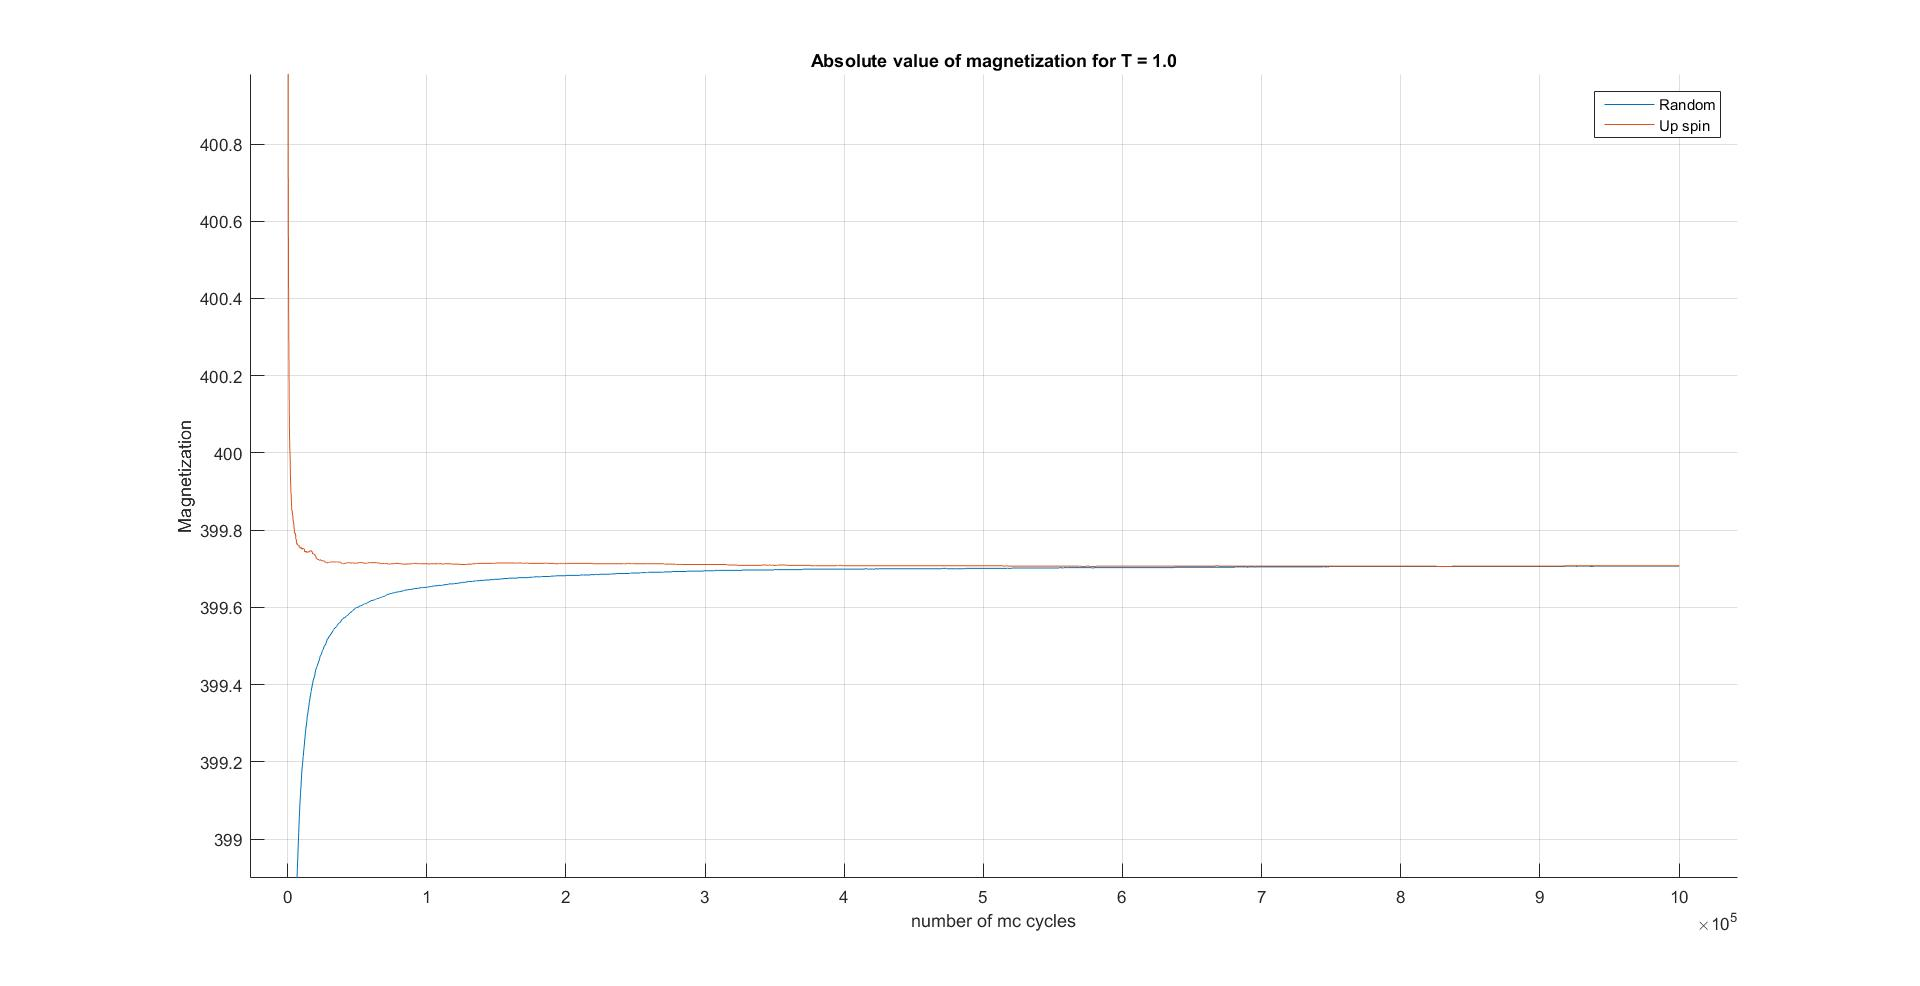
\includegraphics[width=0.7\textwidth]{absmag1T}
}
\caption{Absolute value of magnetization versus Monte Carlo cycles for T = 1.0}
\label{fig:absmag1T}
\end{figure}

\begin{figure}[H]
\centerline{
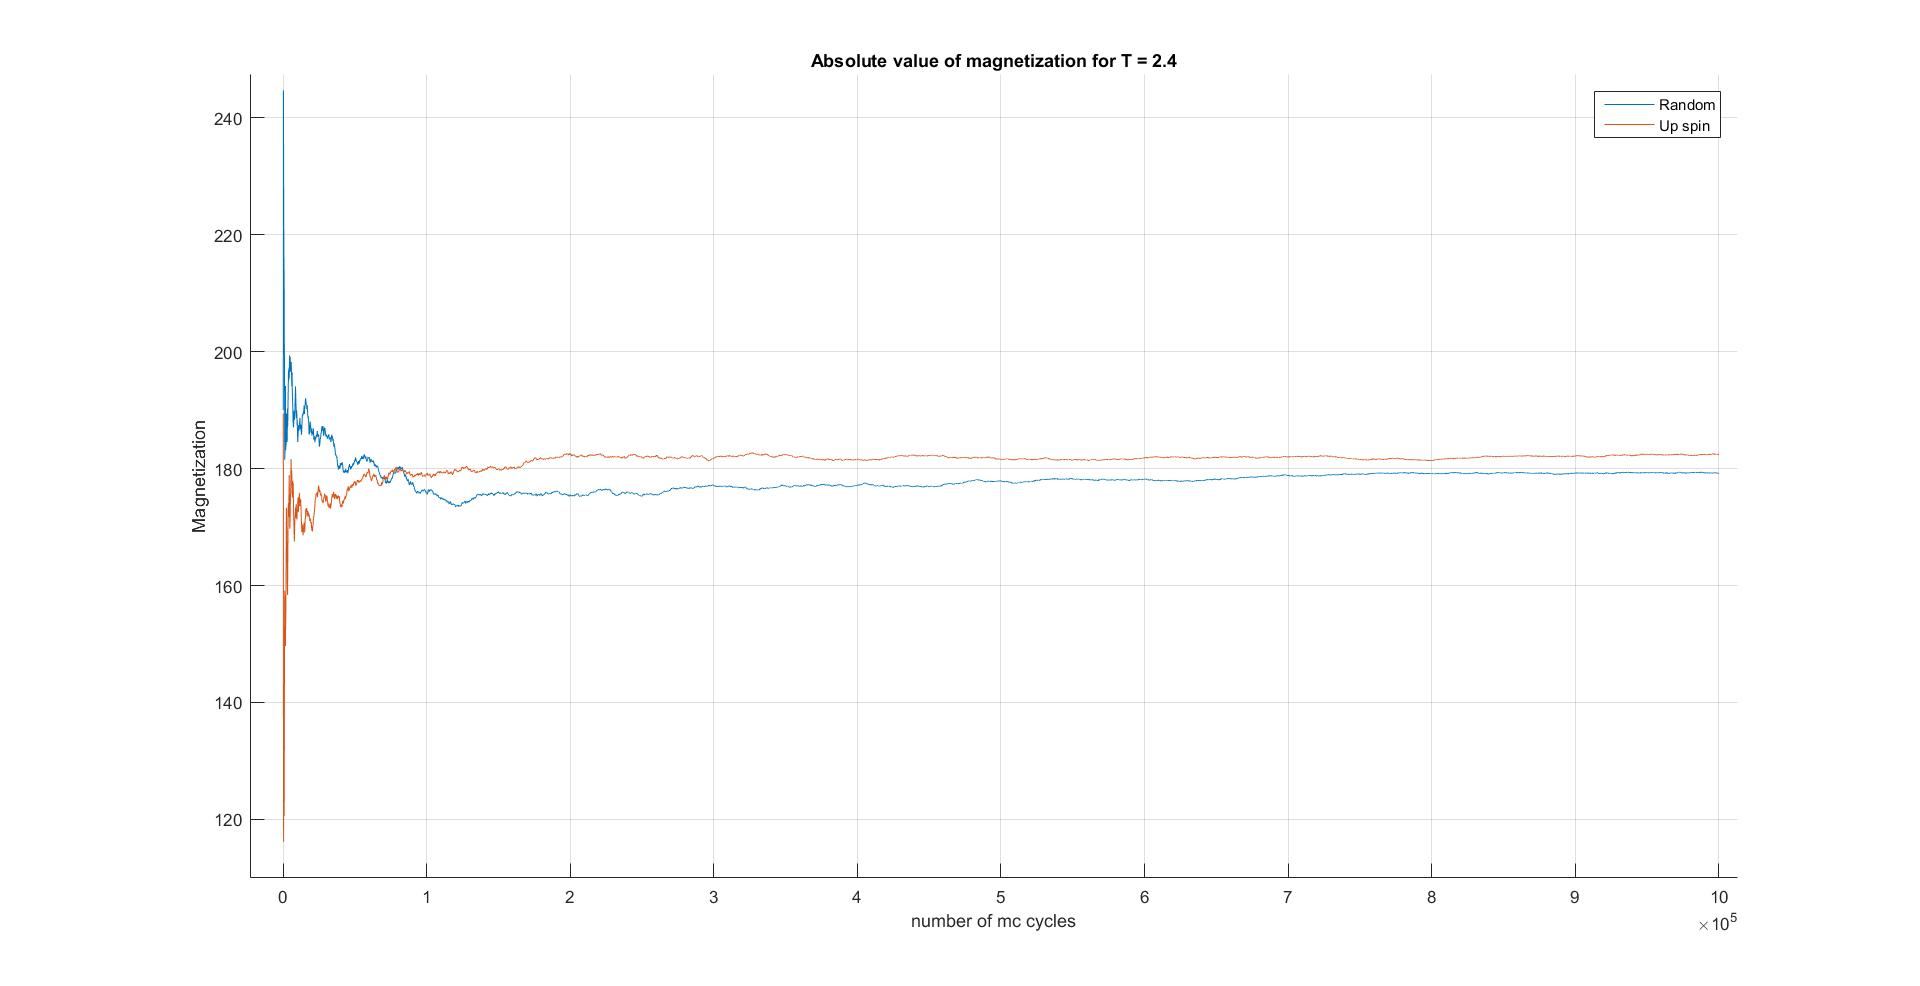
\includegraphics[width=0.7\textwidth]{absmag24T}
}
\caption{Absolute value of magnetization versus Monte Carlo cycles for T = 2.4}
\label{fig:absmag24T}
\end{figure}
\begin{figure}[H]
\centerline{
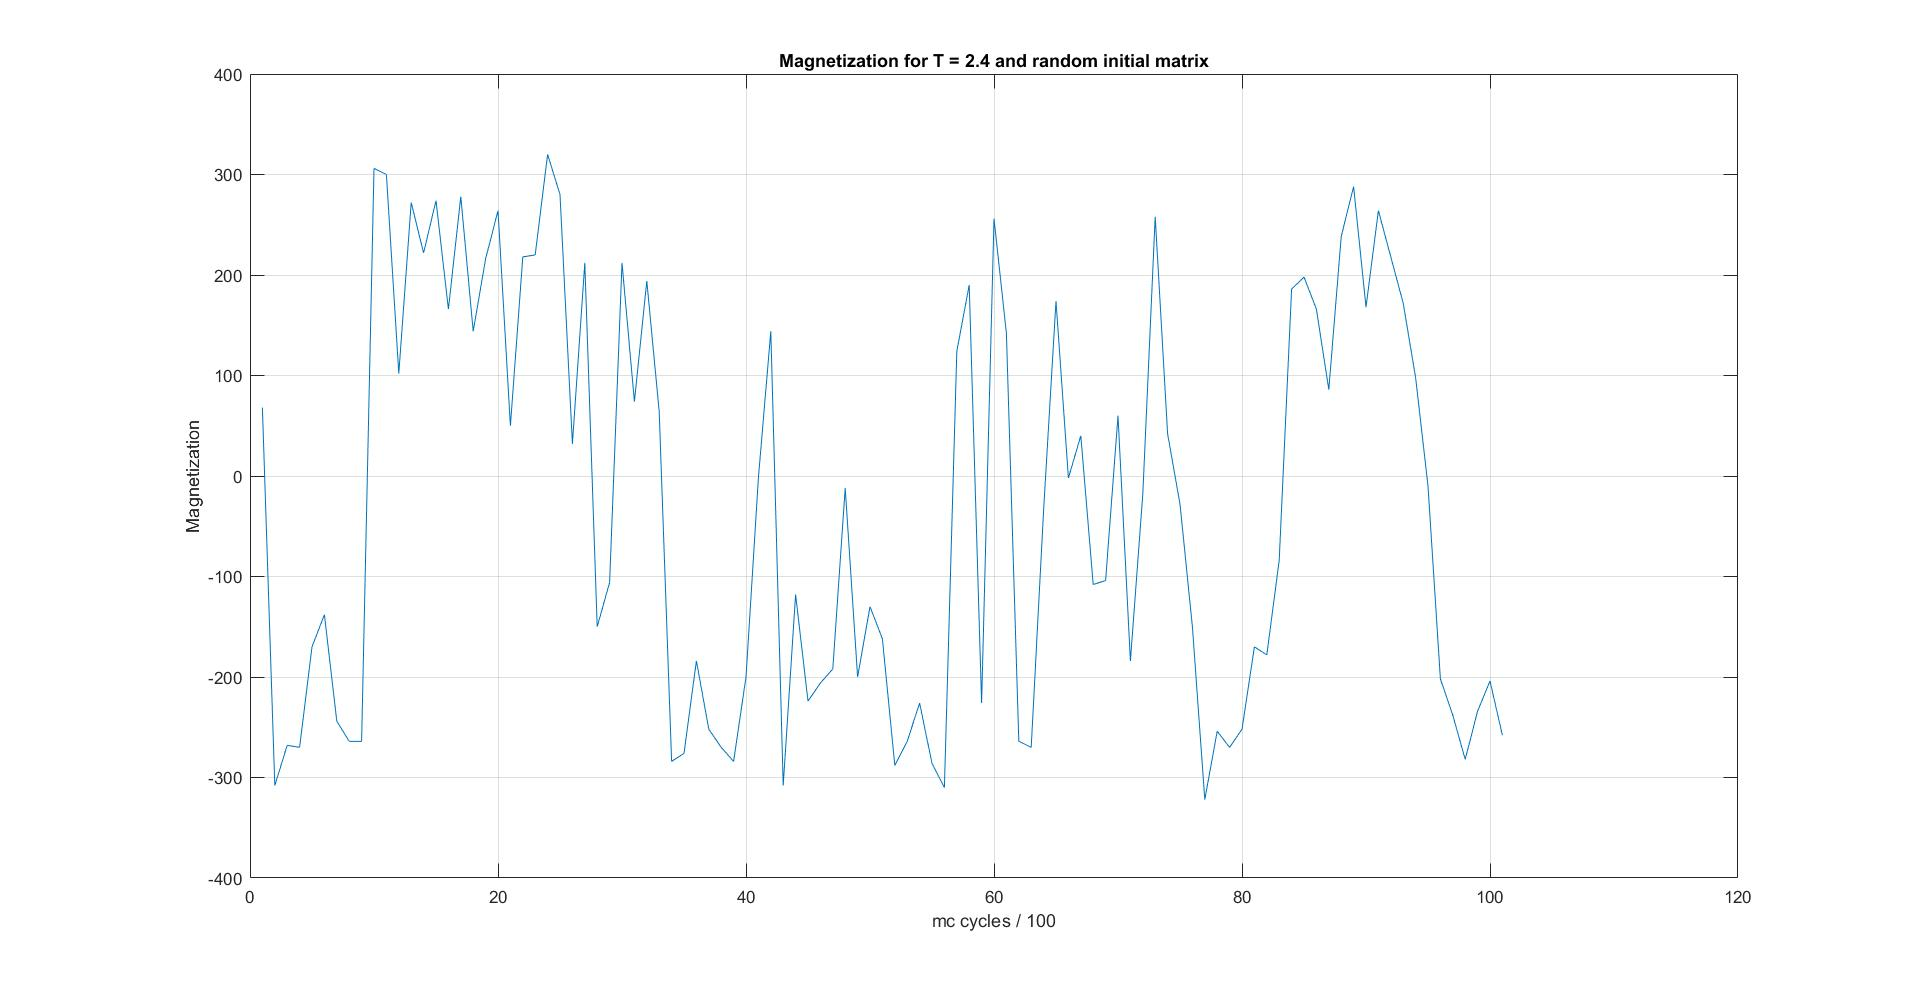
\includegraphics[width=0.7\textwidth]{magnetizationT24random}
}
\caption{Mean magnetization versus Monte Carlo cycles for T = 2.4}
\label{fig:mag24T}
\end{figure}
\begin{figure}[H]
\centerline{
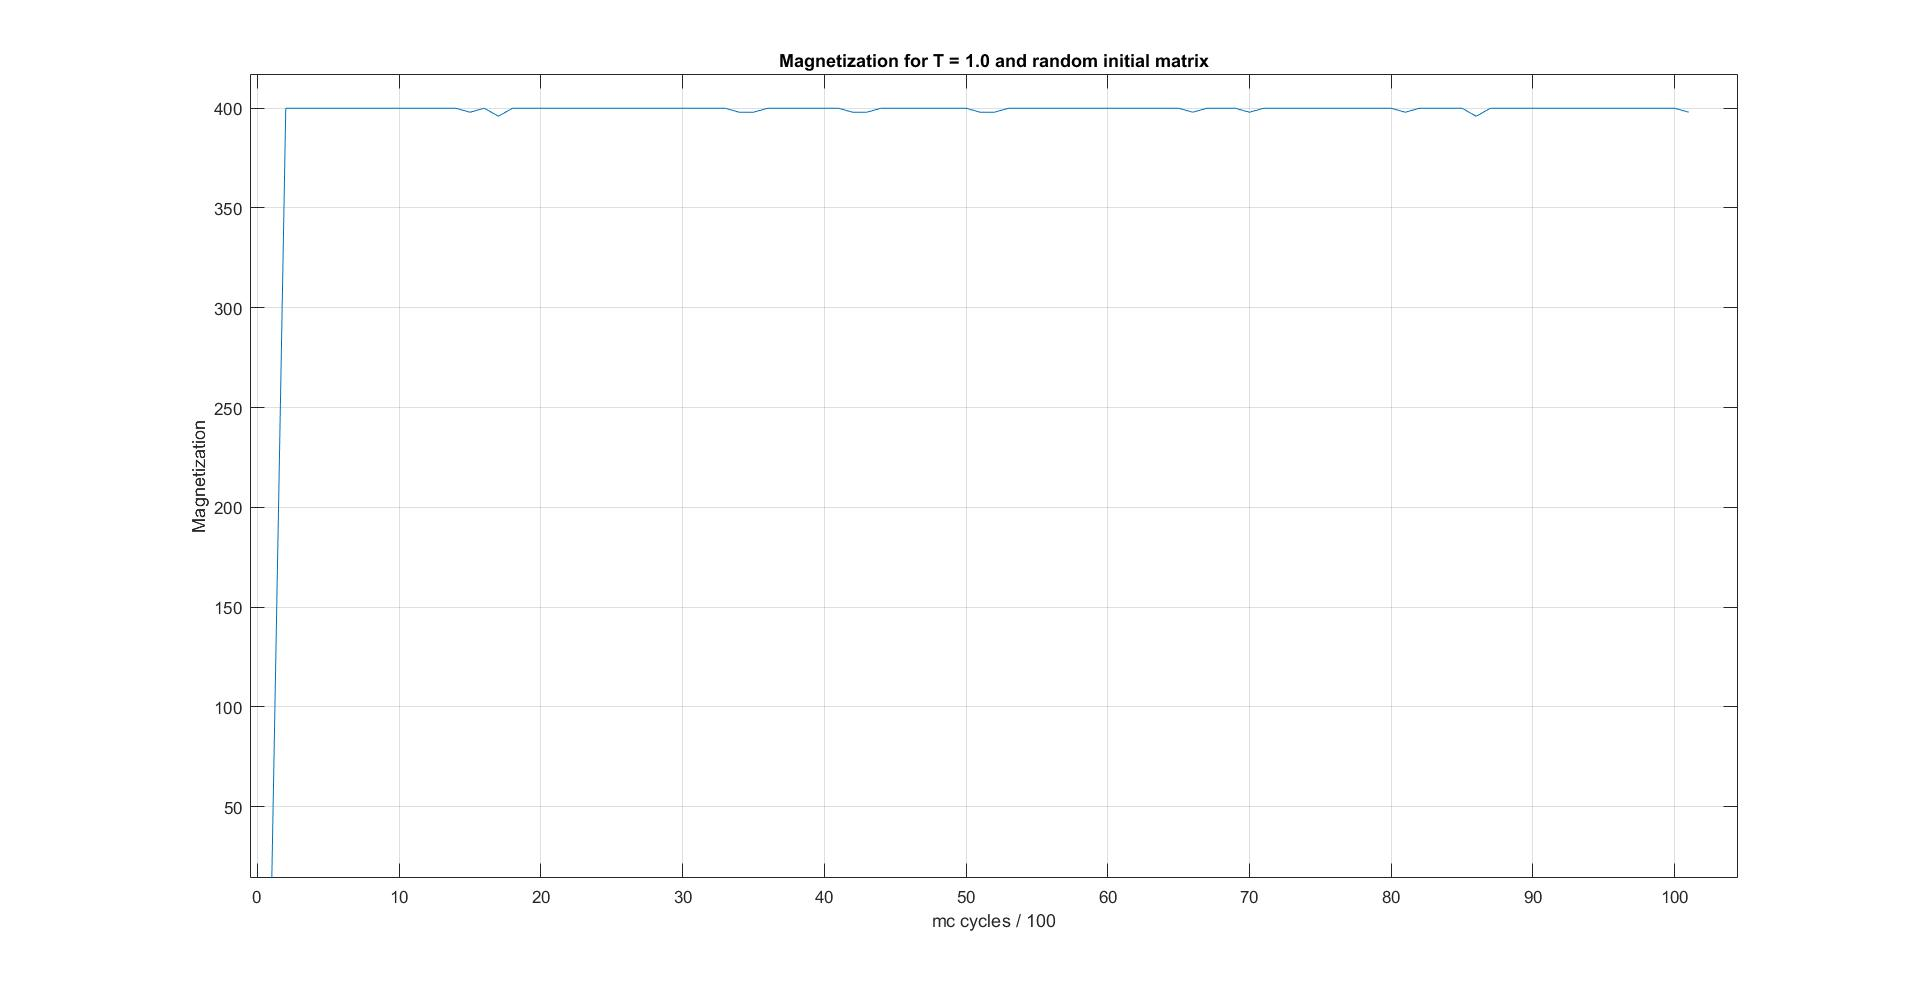
\includegraphics[width=0.7\textwidth]{magnetizationT1random}
}
\caption{Mean magnetization versus Monte Carlo cycles for T = 1.0}
\label{fig:mag1T}
\end{figure}

\noindent One can see from \figref{energy1T}, \figref{energy24T}, \figref{absmag1T} and \figref{absmag24T} that the mean energy and magnetization approaches its equilibrium state. There are fluctuations after the mean energy and magnetization has reached it's equilibrium state, but the value seems to jump back to to the equilibrium state quickly. The values become more unstable when $T = 2.4$, and also the value of the equilibrium state is changed. The number of Monte Carlo cycles needed to hit equilibrium is different for different temperatures, but the initial matrix that is used do not seem to affect the time it takes to reach equilibrium. Looking at \figref{mag24T} and \figref{mag1T}, one can observe that without the absolute value, the magnetization fluctuates quite a lot. Keep in mind that the last two figures are plotted every 100th Monte Carlo cycle. By plotting every Monte Carlo cycle, the graph looked too chaotic to interpret. The tables below shows how many Monte Carlo cycles are needed to reach an equilibrium state for the energy and the magnetization:

\begin{table}[H]
\caption{EQ values for energy} \label{tab:table2}
\centerline{
\begin{tabular}{|c|c|c|c|}
\hline
Orientation & Temperature & EQ state & max MC cycles needed\\
\hline
Random & 1.0 & -790.881 & $2*10^4$\\
\hline
Random & 2.4 & -496.494 & $3*10^5$\\
\hline
Up spin & 1.0 & -798.96 & $2*10^4$\\
\hline
Up spin & 2.4 & -493.996 & $3*10^5$\\
\hline
\end{tabular}
}
\end{table}

\begin{table}[H]
\caption{EQ values for magnetization} \label{tab:table3}
\centerline{
\begin{tabular}{|c|c|c|c|}
\hline
Orientation & Temperature & EQ state & max MC cycles needed\\
\hline
Random & 1.0 & 398.762 & $6*10^5$\\
\hline
Random & 2.4 & 165.209 & $2*10^5$\\
\hline
Up spin & 1.0 & 399.732 & $10^5$\\
\hline
Up spin & 2.4 & 176.087 & $2*10^5$\\
\hline
\end{tabular}
}
\end{table}

\begin{figure}[H]
\centerline{
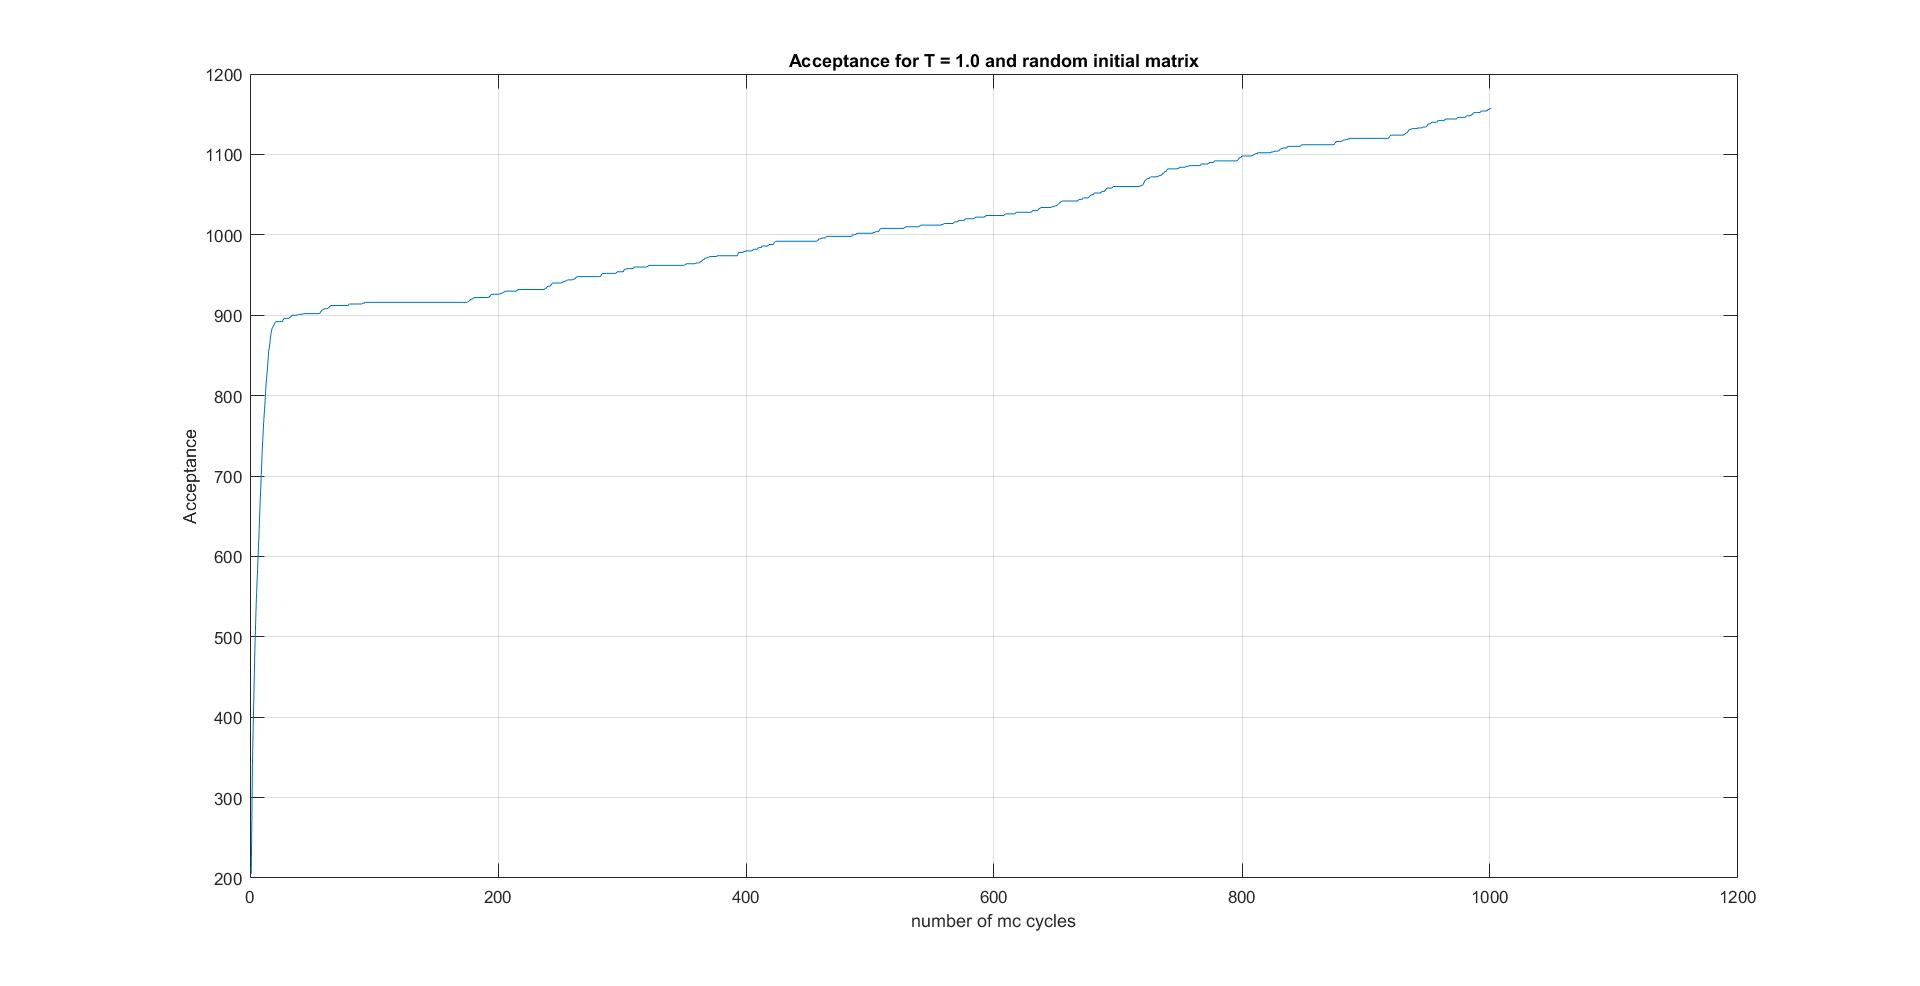
\includegraphics[width=0.7\textwidth]{acceptanceMCT1random}
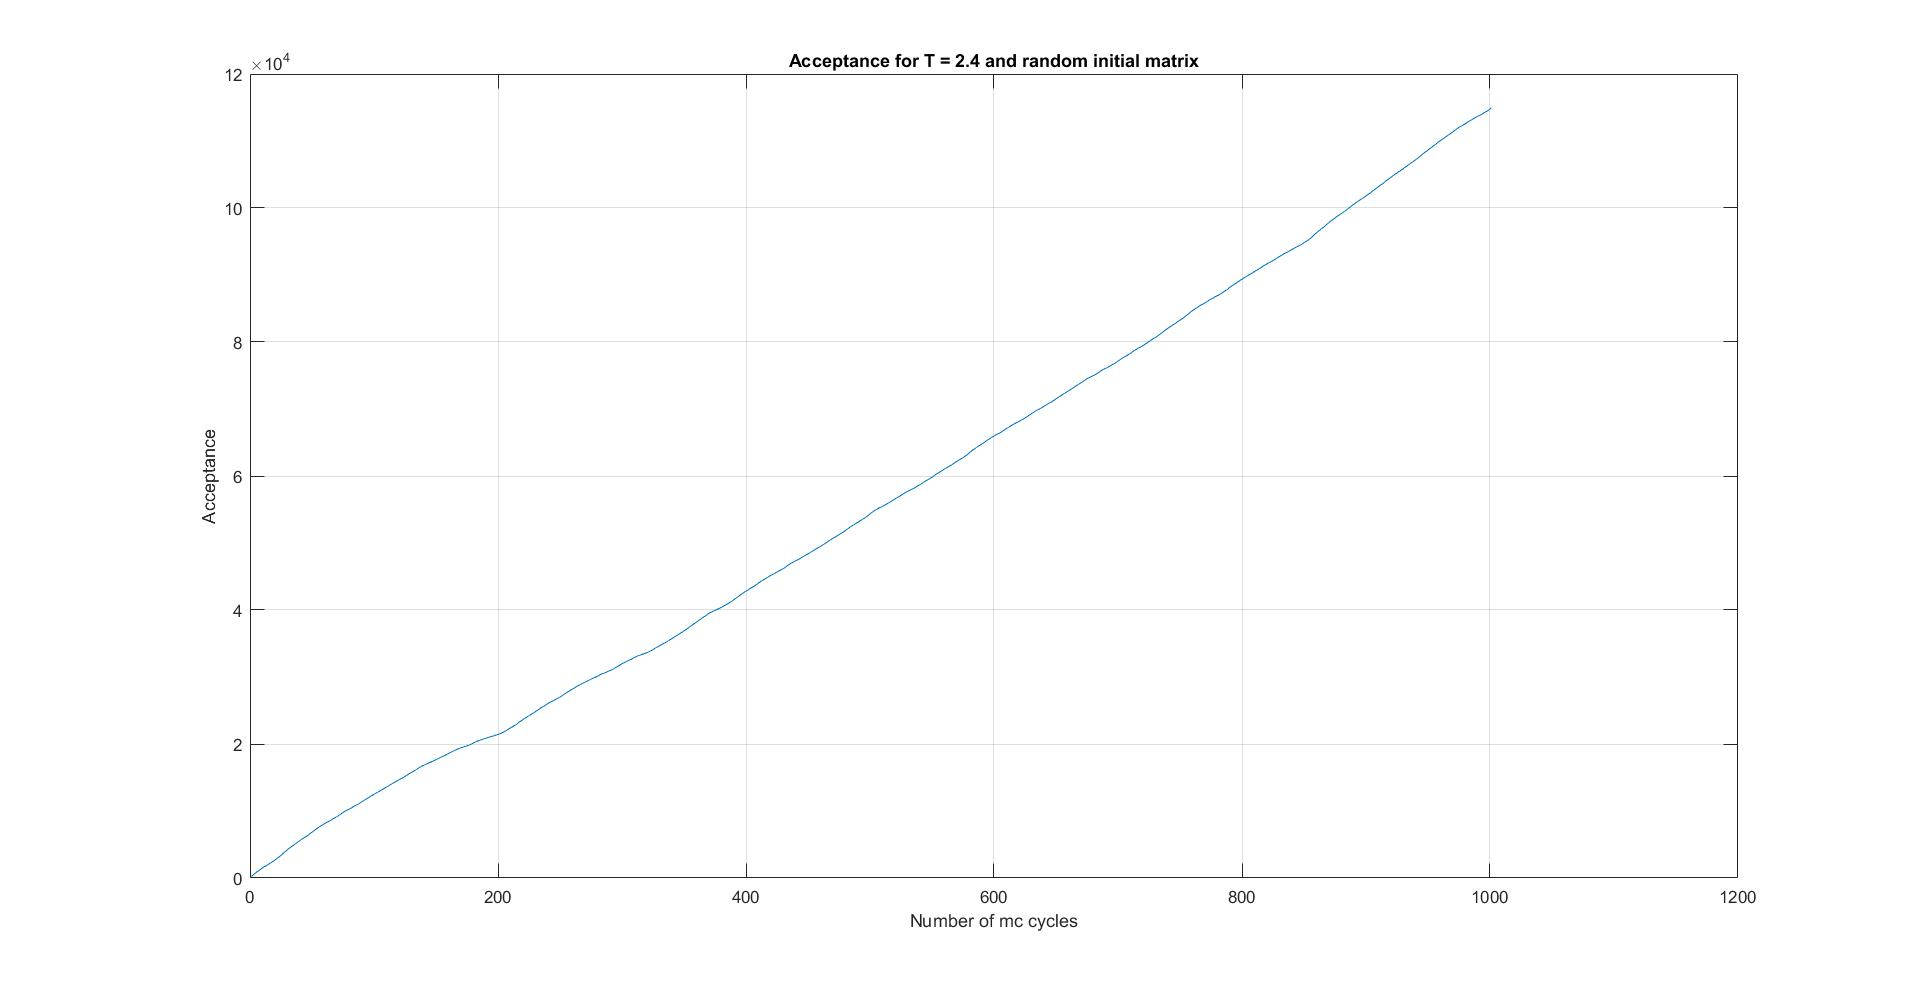
\includegraphics[width=0.7\textwidth]{acceptanceMCT24random}
}
\caption{Acceptance versus Monte Carlo cycles for T = 1.0 and T = 2.4 with a random initial matrix}
\label{fig:acceptancerandom}
\end{figure}

\begin{figure}[H]
\centerline{
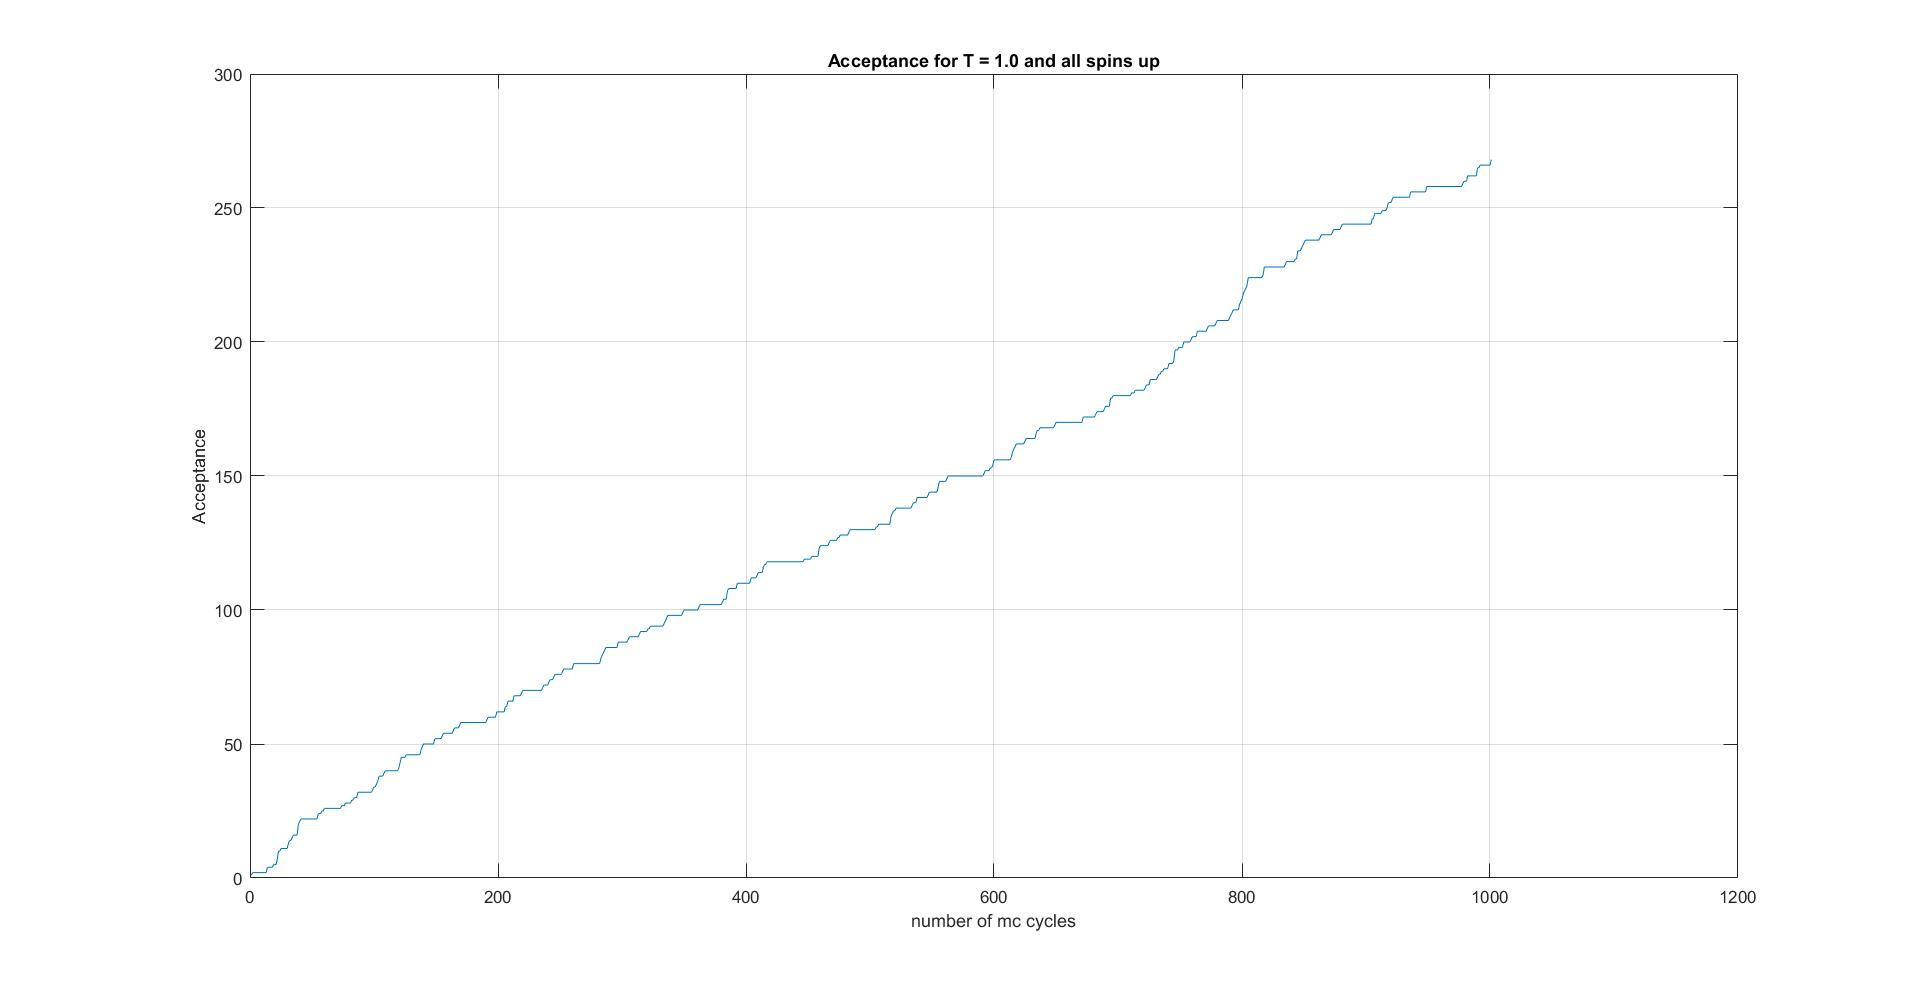
\includegraphics[width=0.7\textwidth]{acceptanceMCT1upspin}
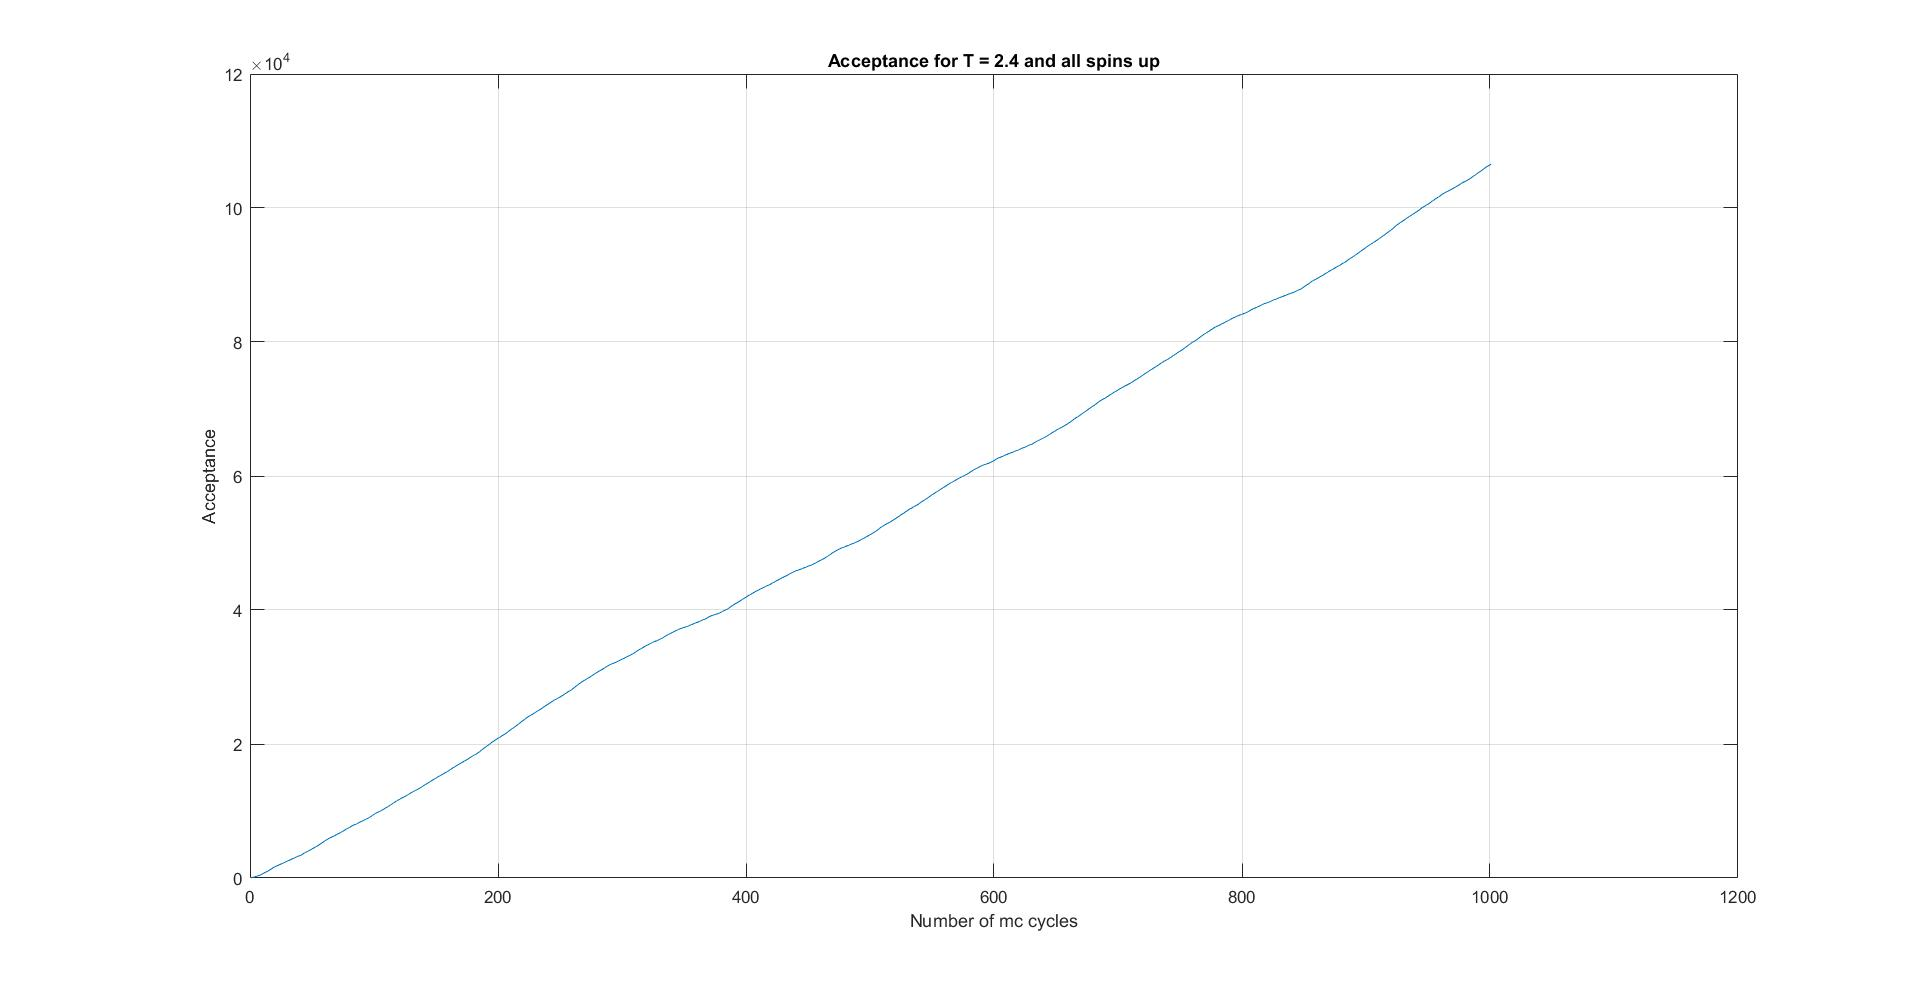
\includegraphics[width=0.7\textwidth]{acceptanceMCT24upspin}
}
\caption{Acceptance versus Monte Carlo cycles for T = 1.0 and T = 2.4 with initial spin upwards}
\label{fig:acceptanceupspin}
\end{figure}

\begin{figure}[H]
\centerline{
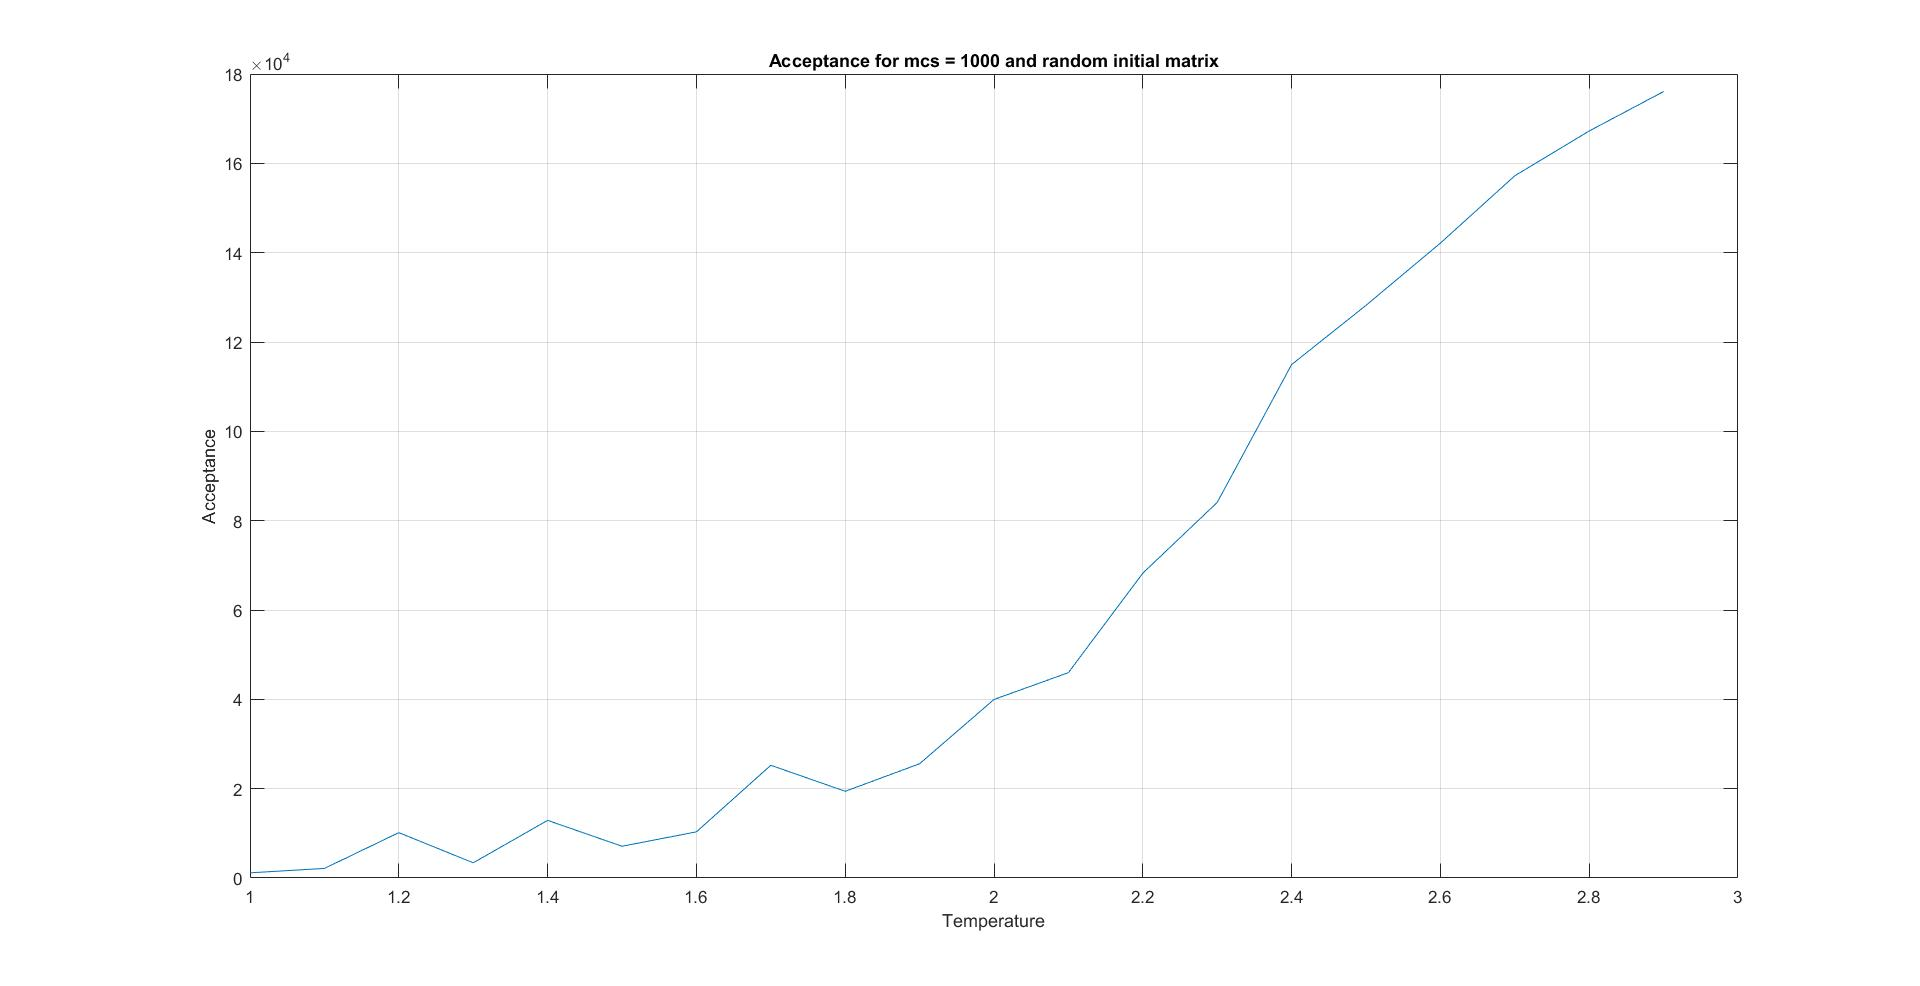
\includegraphics[width=0.7\textwidth]{acceptanceVStrandom}
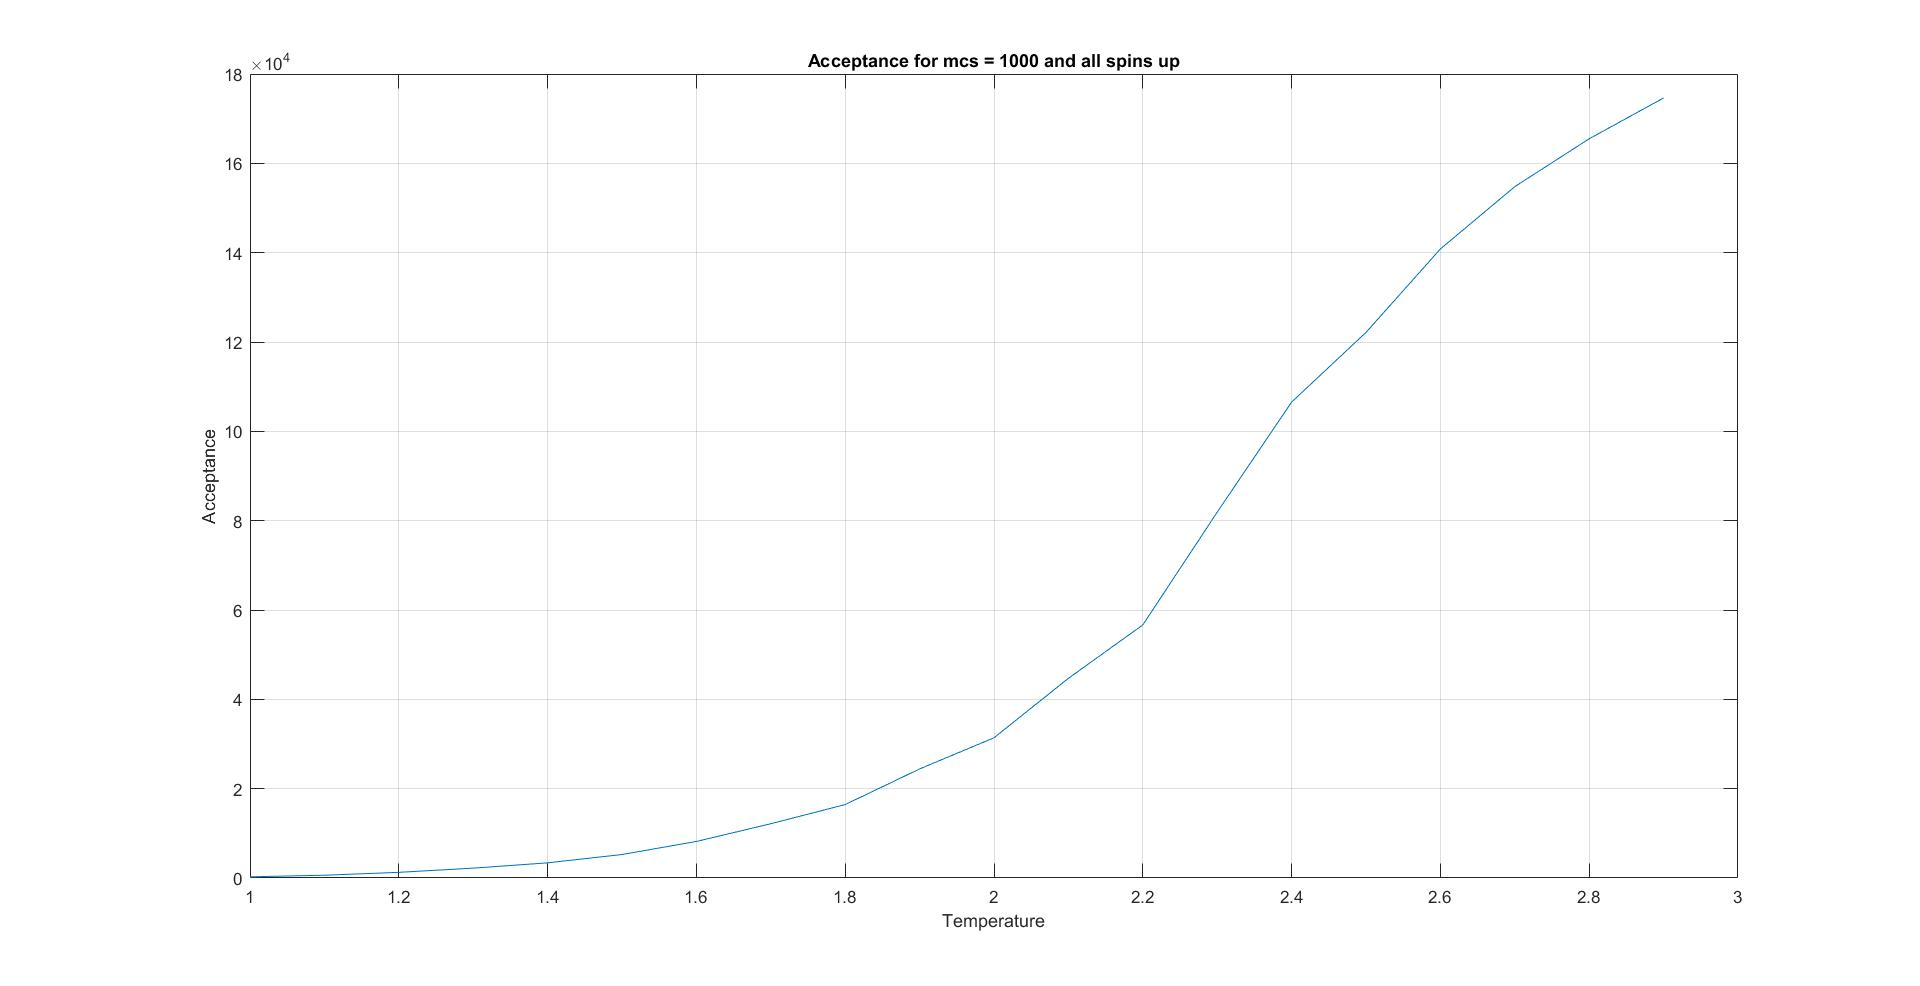
\includegraphics[width=0.7\textwidth]{acceptanceVStupspin}
}
\caption{Acceptance versus temperature for a random initial matrix and with initial spin upwards}
\label{fig:acceptancetemp}
\end{figure}

\noindent Acceptance is apparently dependent on both temperature and the initial state of the spins. From figure \figref{acceptancerandom} one can observe that with higher temperature, the number of accepted values (y-axis) increase by a factor of $10$. For $T = 1.0$ and random initial matrix, one can also observe that the acceptance spikes for few Monte Carlo cycles. 
\\
If the initial spins are all upwards like in \figref{acceptanceupspin}, the acceptance becomes more linear. The line for $T = 1.0$ is more squiggly than the straighter line for $T = 2.4$. The ladder does not spike for few Monte Carlo cycles.
\\
From \figref{acceptancetemp}, one can observe that the curves increase exponentially towards $T = 2.4$, where it flattens. The curve based on a randomly generated initial matrix is uneven at low temperatures, but smooths out when $T$ increases. When the initial matrix only consist positive spins, the curve is smooth throughout. These two graphs are plotted to a maximum temperature of $3.0$, so one would have an idea of how the acceptance would evolve after $T = 2.4$. 

\begin{figure}[H]
\centerline{
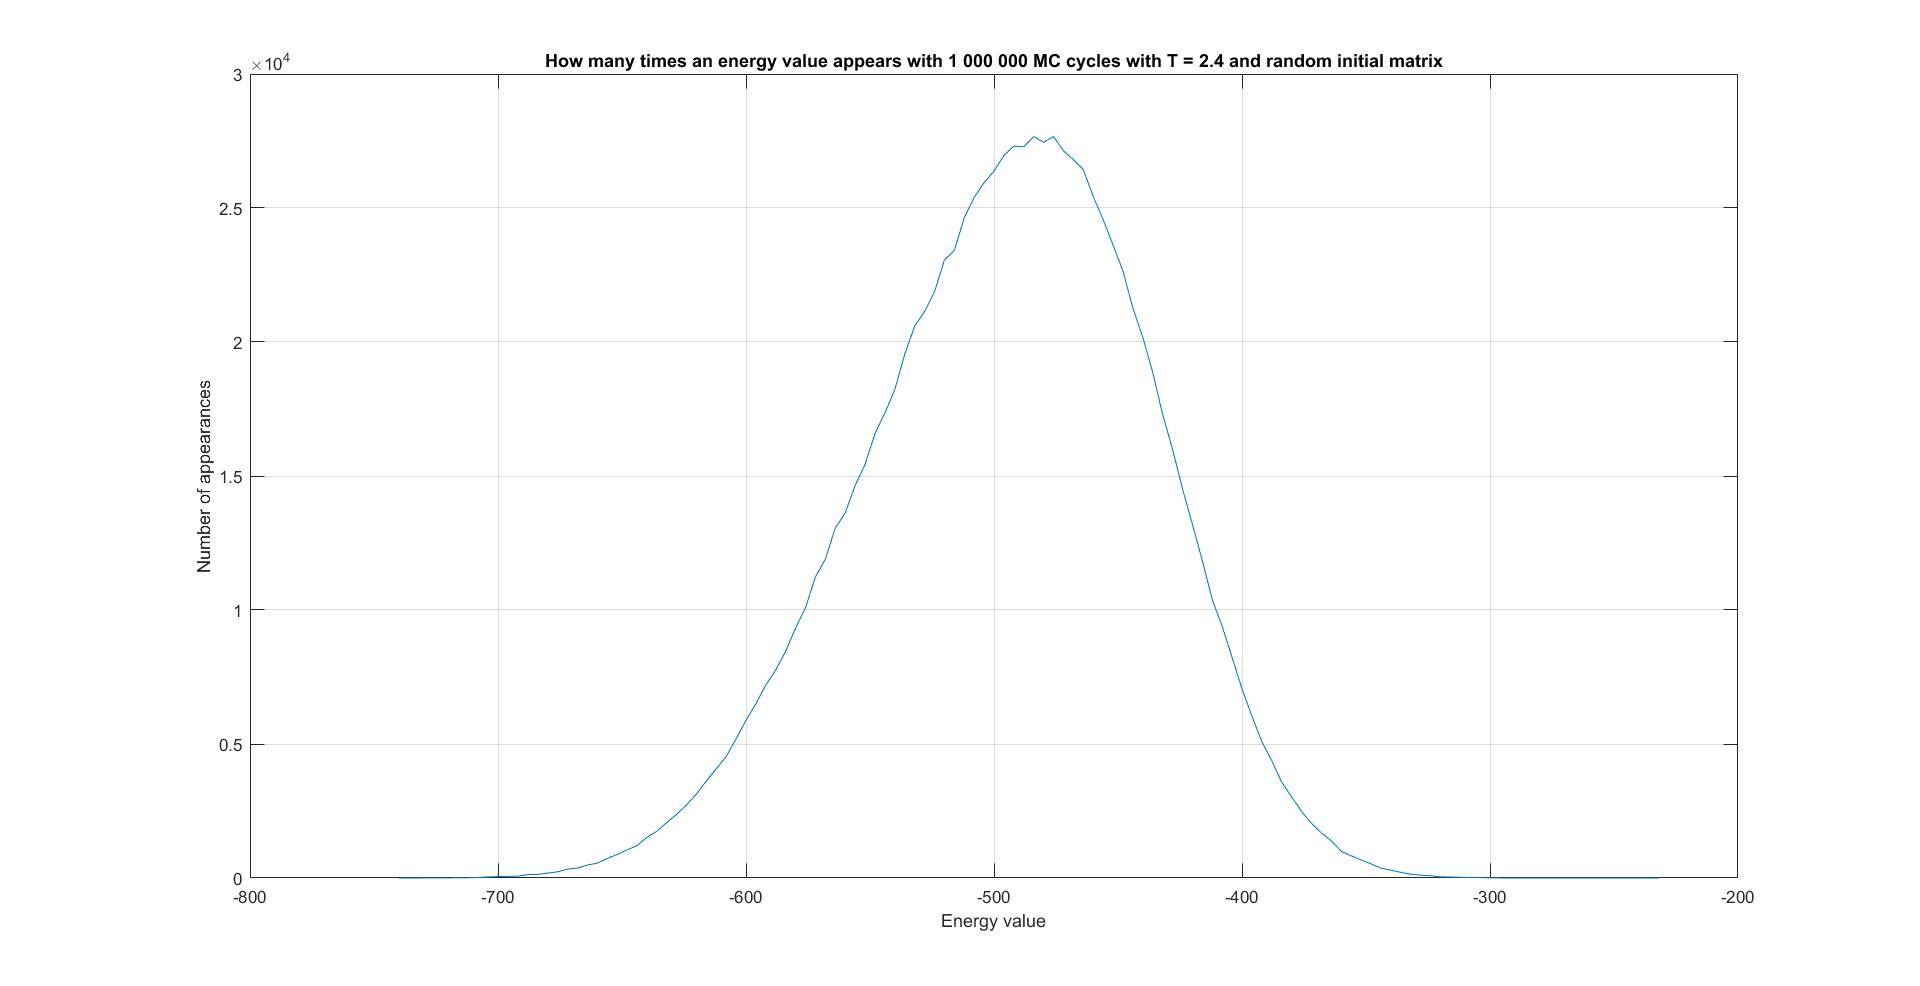
\includegraphics[width=0.7\textwidth]{energyappearanceT24random}
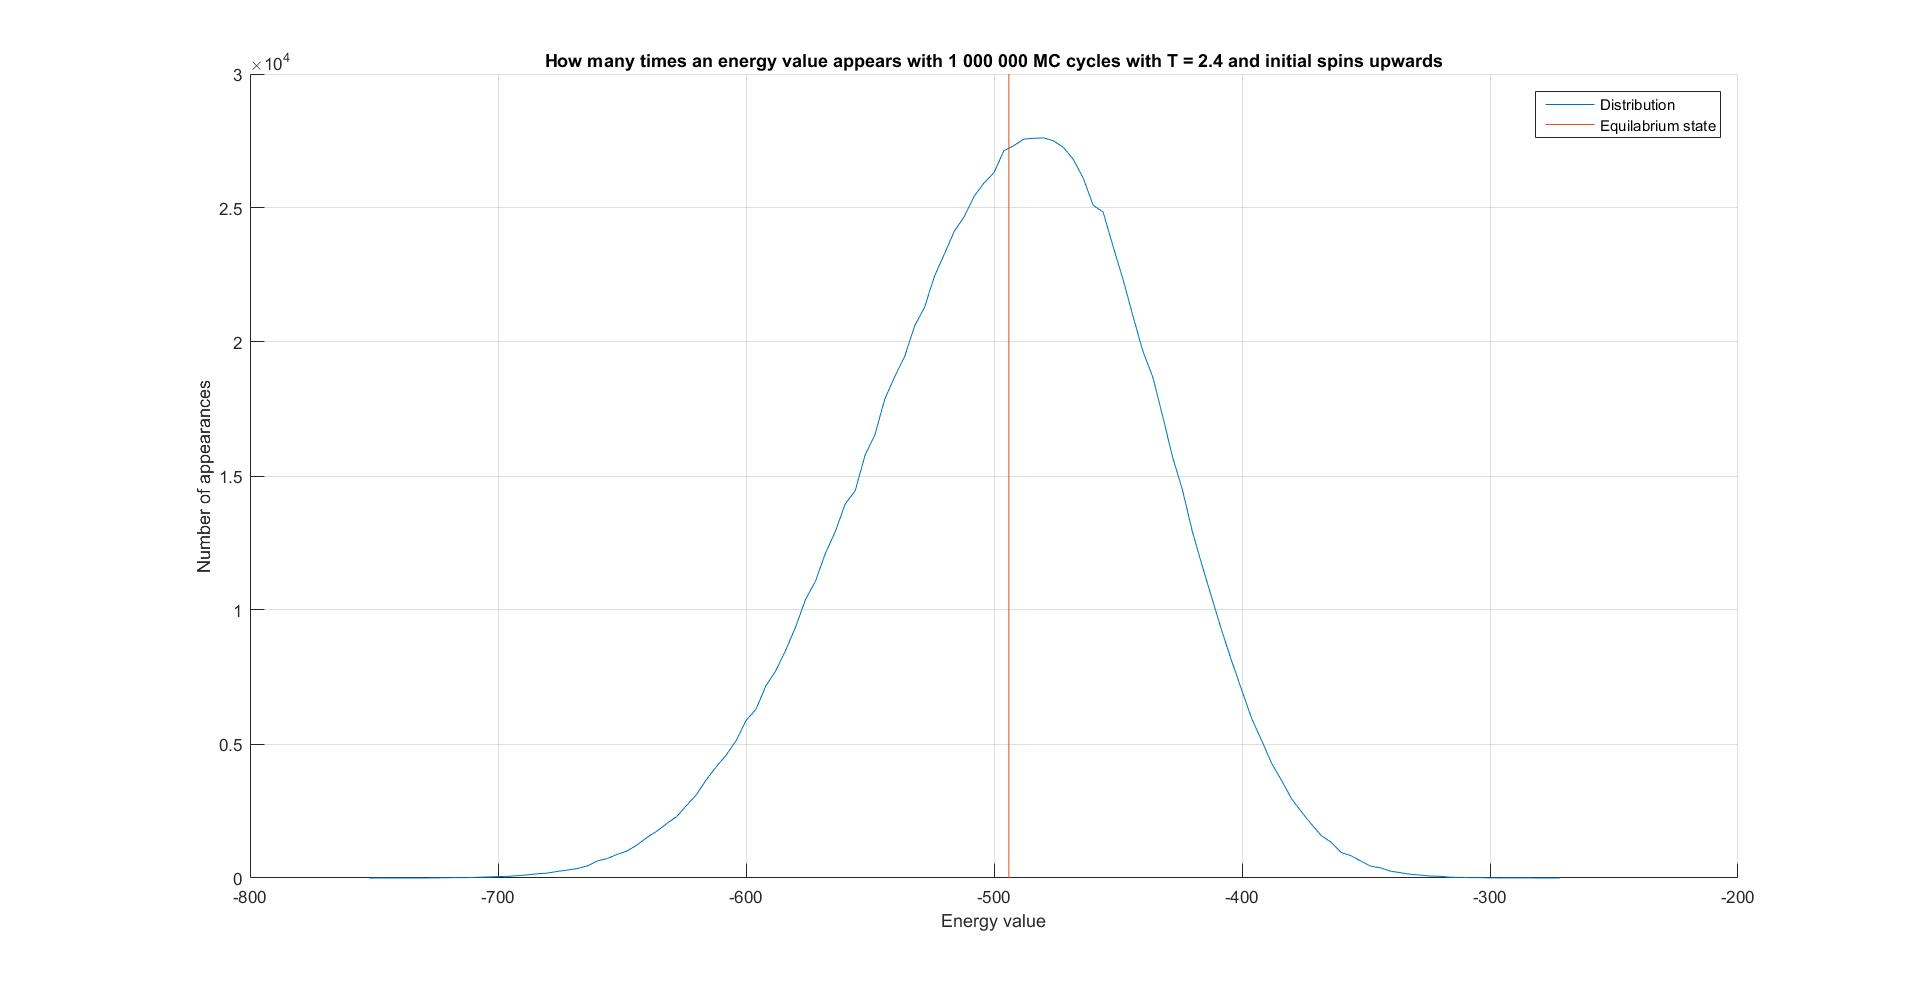
\includegraphics[width=0.7\textwidth]{energyappearanceT24upspin}
}
\caption{Number of appearances per energy value for a random initial matrix and with initial spin upwards when T = 2.4}
\label{fig:energyappearance}
\end{figure}
\begin{figure}[H]
\centerline{
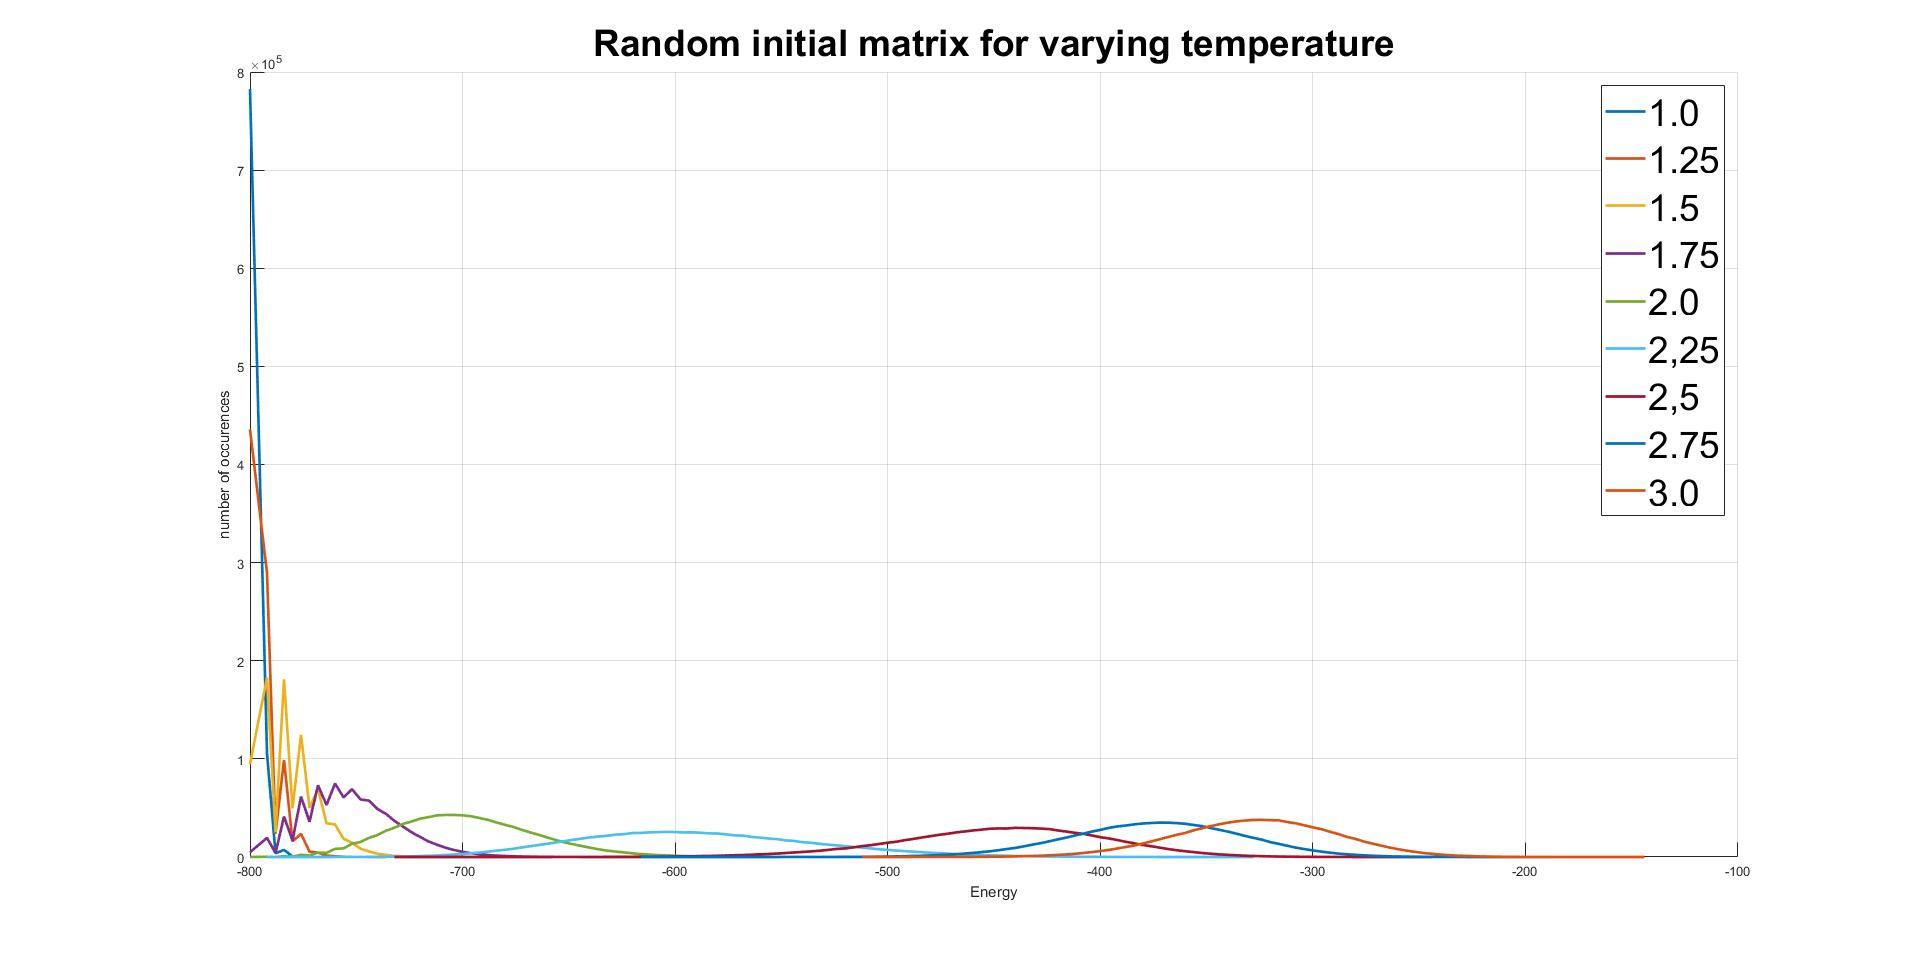
\includegraphics[width=0.7\textwidth]{energyappearanceALL}
}
\caption{Number of appearances per energy value for a random initial matrix and multiple temperatures}
\label{fig:energyappearanceALL}
\end{figure}

\noindent One can observe from \figref{energyappearance} that the curves are slightly skewed towards the higher energy values. The curve is bell shaped and has the majority of values to the left of its equilibrium. The equilibrium states for the lattice at temperature $T = 2.4$ which are $random = -497$ and $Up spin = -493$. From \figref{energyappearanceALL}, one can observe that with higher temperature, the broader the distribution of energy becomes which is reflected in Table \ref{tab:table4}. When the distribution broadens, the variance (and standard deviation) increase.\\

\noindent With a randomly generated initial matrix, the variance computed in c++ for $T = 2.4$ is $3226.62$. The calculated variance from the energy becomes $3226.9$ for $10^6$ MC cycles (calculated in MatLab script "howmanytimes.m"). This gives great confidence in the variance. With fewer Monte Carlo cycles, the two variances calculated does not correlate as well. Variances for other temperatures are shown in the table below and one can observe that the variance increase towards $2.25$ and then decreases. The variance actually peaks at $2.24$, but the values below are calculated with too low resolution to see that:
\begin{table}[H]
\caption{Variance for different temperatures for the entire lattice} \label{tab:table4}
\centerline{
\begin{tabular}{|c|c|}
\hline
  Temperature & Variance\\
\hline
  T=1.0 & 9.09764\\
\hline
  T=1.25 & 51.7348\\
\hline
  T=1.50 & 177.7472\\
\hline
  T=1.75 & 478.188\\
\hline
  T=2.0 & 1152.904\\
\hline 
  T=2.25 & 3158.504\\
\hline 
  T= 2.50 & 2473.664\\
\hline 
  T=2.75 & 1700.996\\
\hline
  T=3.0 & 1446.38\\
\hline
\end{tabular}
}
\end{table}

\noindent The run time for higher order lattices increased as the lattice size increased and this is shown in the table below:

\begin{table}[H]
\caption{Run time for different lattice sizes with $10^6$ MC cycles and 20 different temperatures ranging from $T = 2.0$ to $T = 3.0$} \label{tab:table5}
\centerline{
\begin{tabular}{|c|c|}
\hline
  Lattice size & Run time in seconds\\
\hline
  60x60 & 3996.57\\
\hline
  80x80 & 7081.15\\
\hline
  100x100 & 18630.9\\
\hline
\end{tabular}
}
\end{table}

\begin{figure}[H]
\centerline{
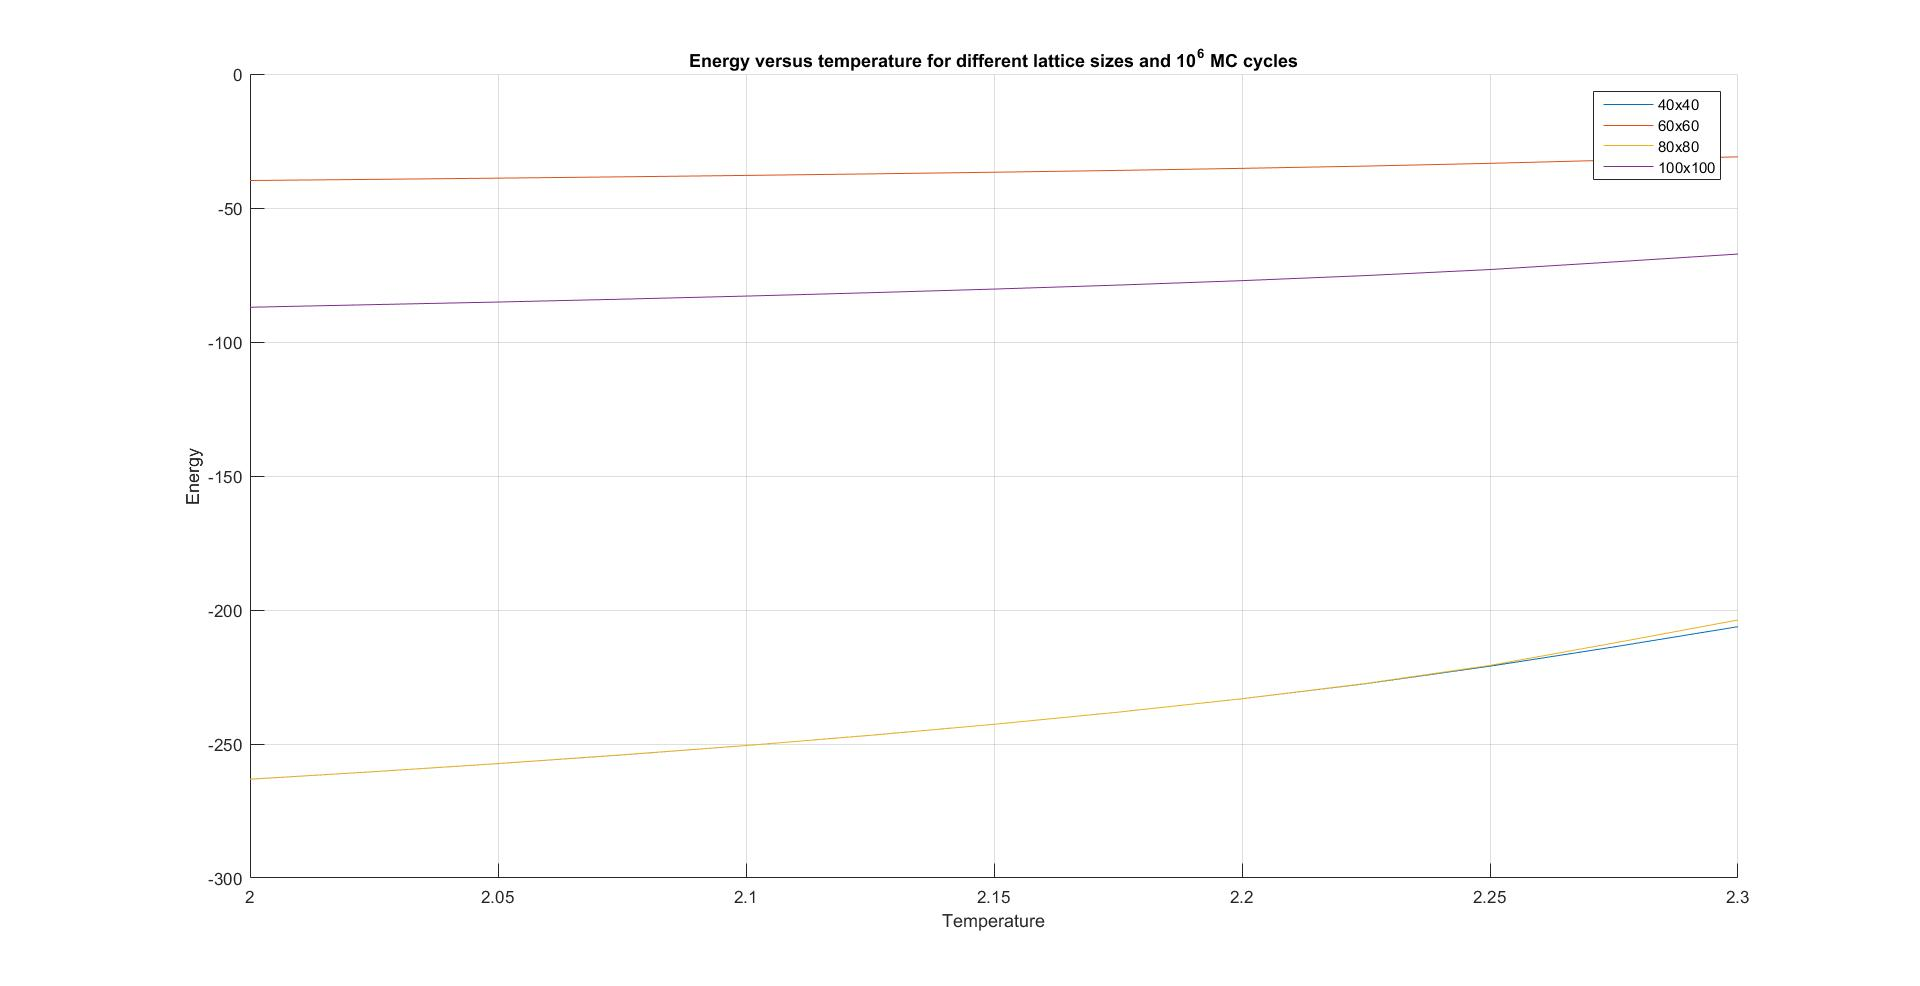
\includegraphics[width=0.7\textwidth]{energyVSt}
}
\caption{Mean energy versus temperature for $10^6$ Monte Carlo cycles for single lattice objects}
\label{fig:energyVSt}
\end{figure}

\begin{figure}[H]
\centerline{
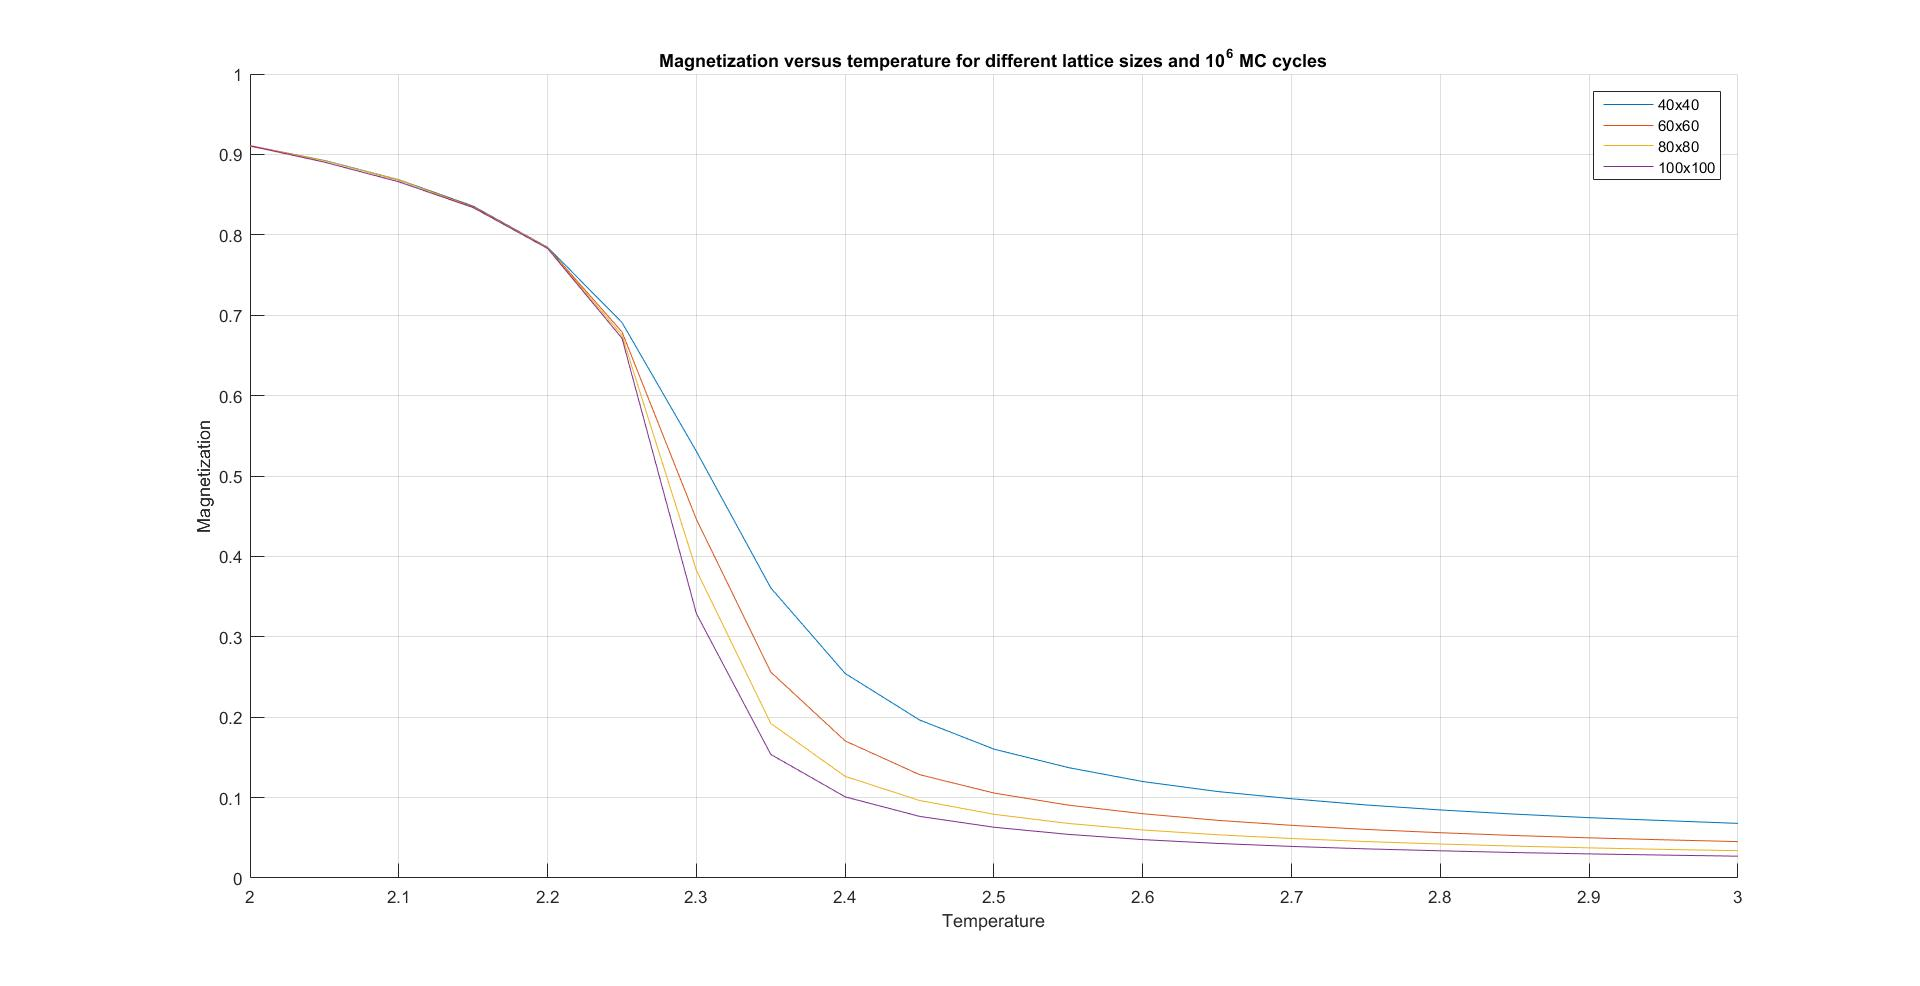
\includegraphics[width=0.7\textwidth]{magnetizationVSt}
}
\caption{Mean magnetization versus temperature for $10^6$ Monte Carlo cycles for single lattice objects}
\label{fig:magVSt}
\end{figure}

\begin{figure}[H]
\centerline{
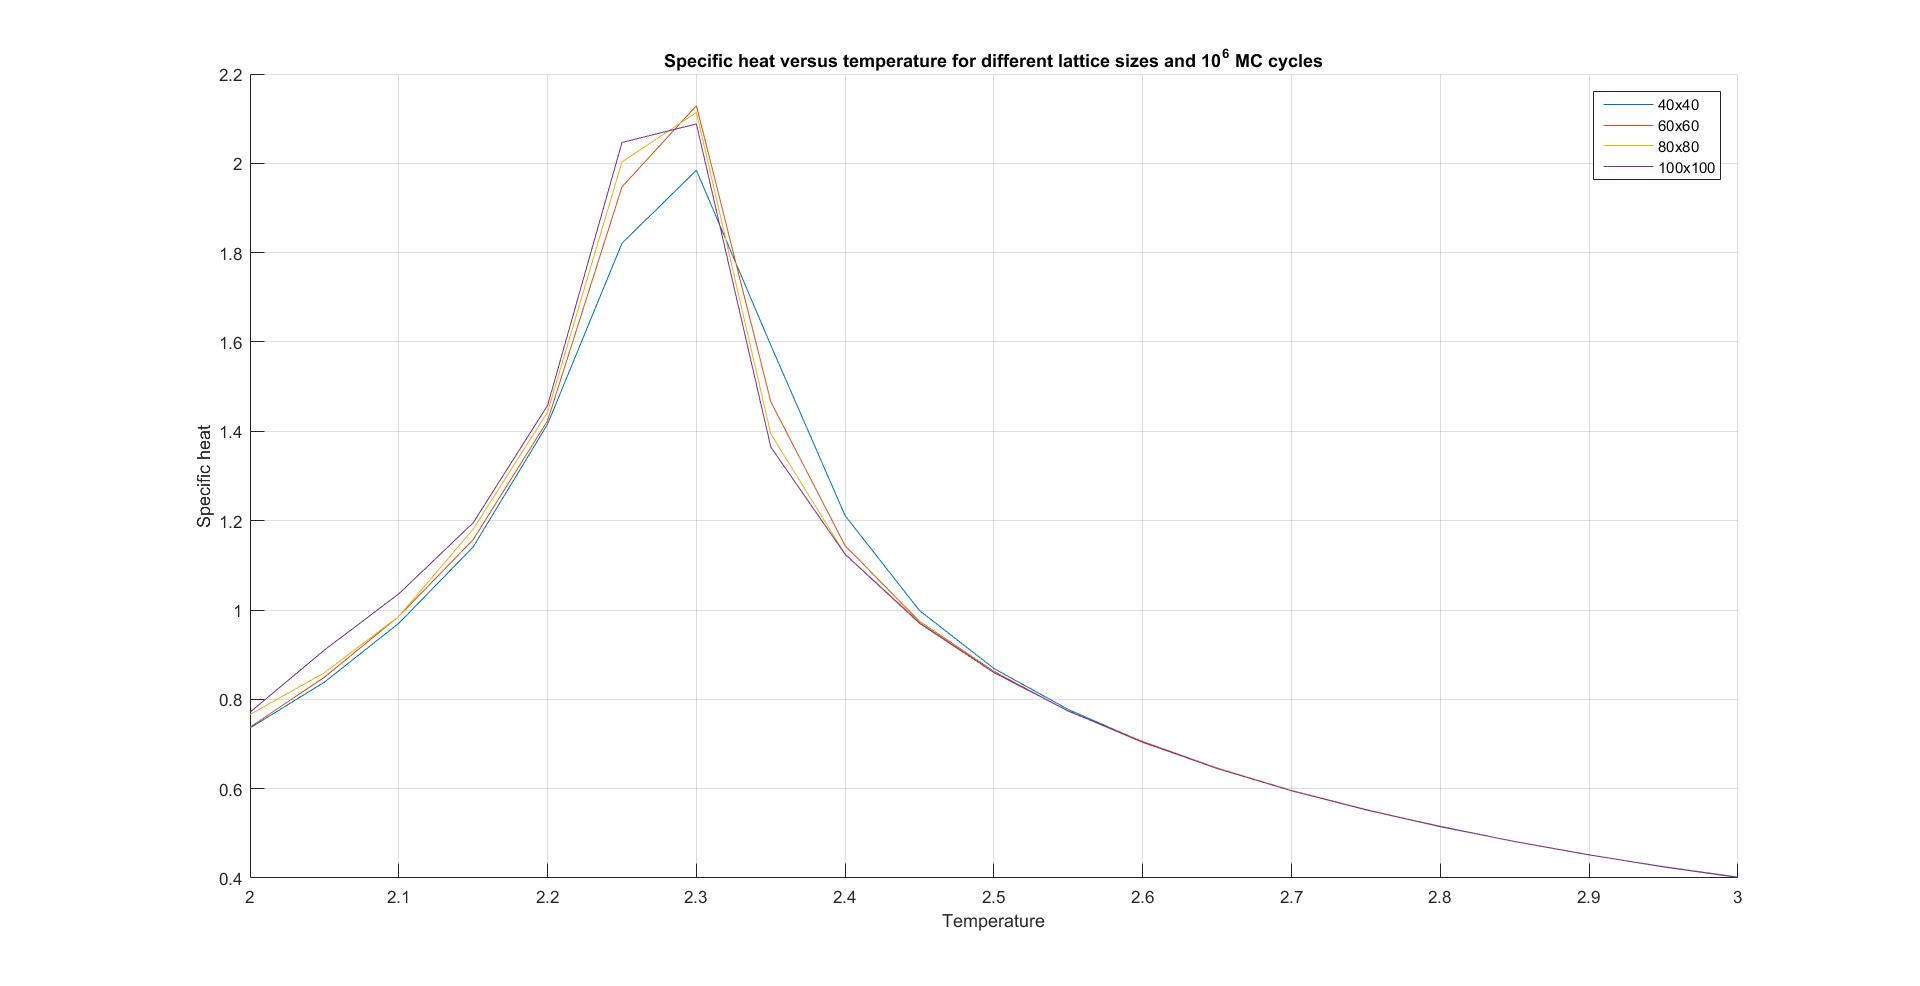
\includegraphics[width=0.7\textwidth]{heatVSt}
}
\caption{Specific heat versus temperature for $10^6$ Monte Carlo cycles for single lattice objects}
\label{fig:heatVSt}
\end{figure}

\begin{figure}[H]
\centerline{
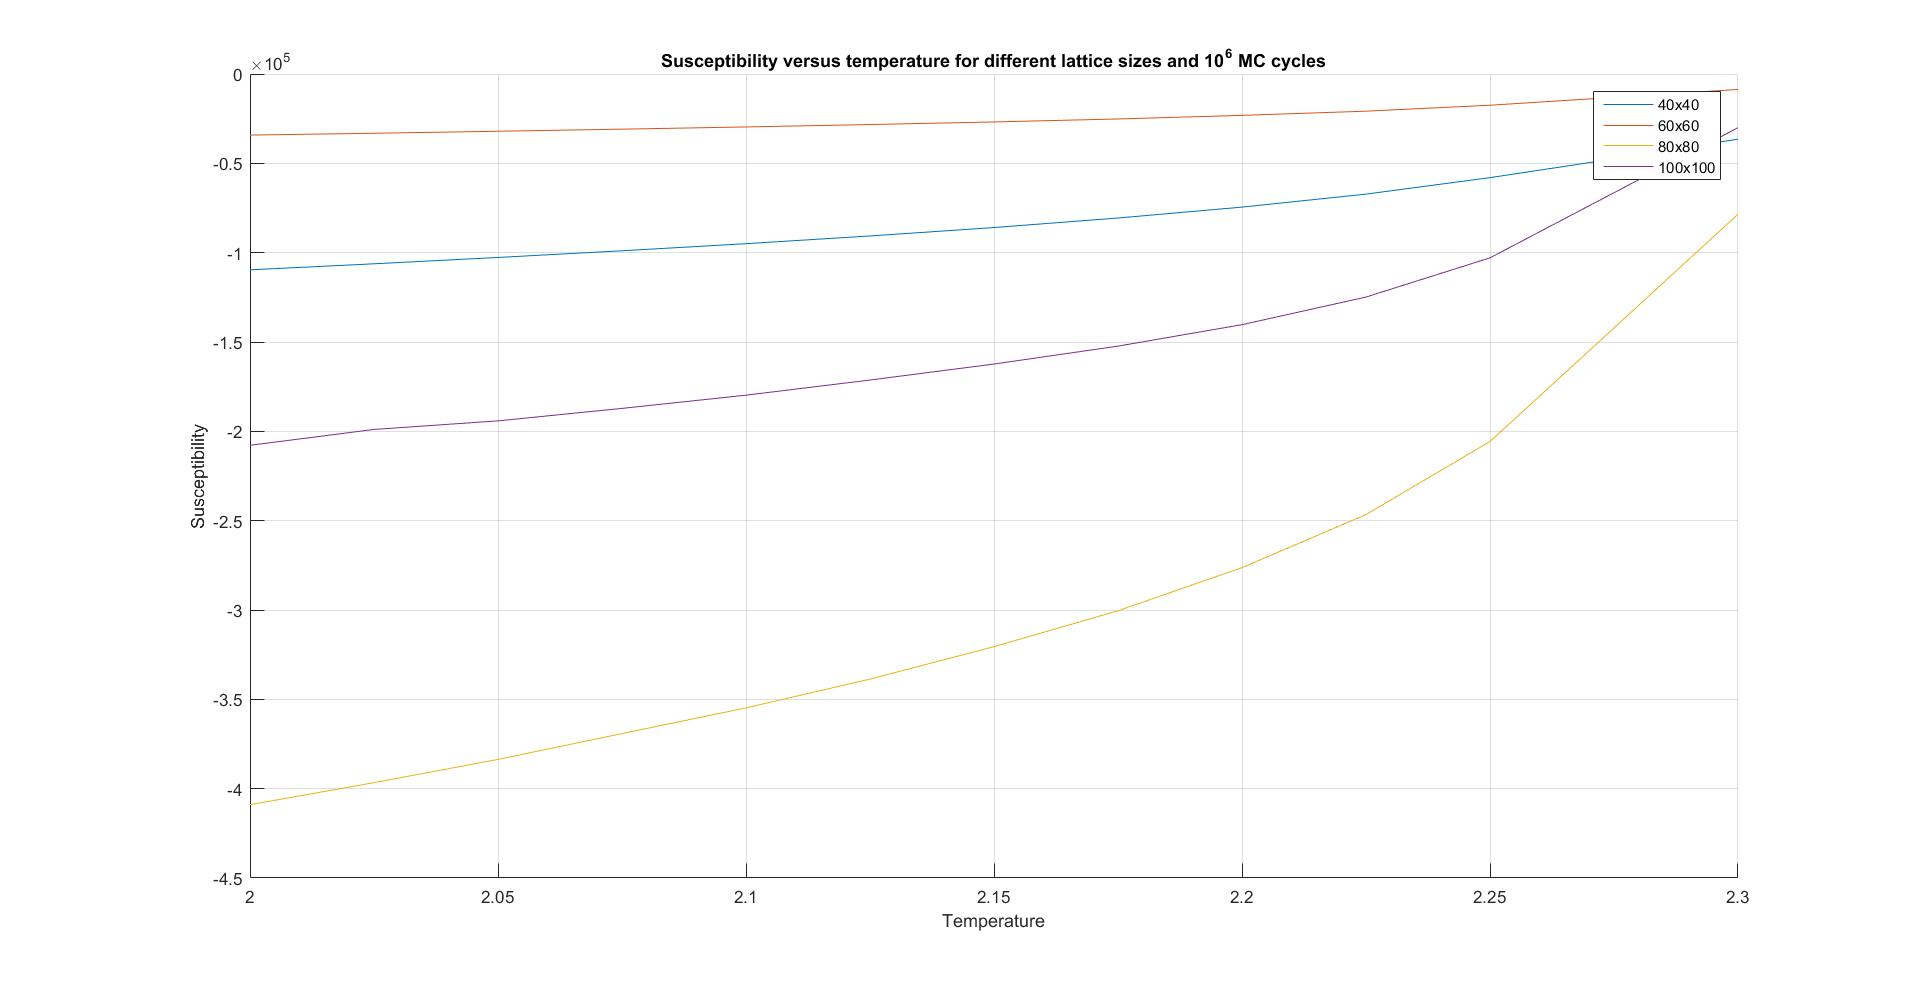
\includegraphics[width=0.7\textwidth]{susceptibilityVSt}
}
\caption{Susceptibility versus temperature for $10^6$ Monte Carlo cycles for single lattice objects}
\label{fig:susVSt}
\end{figure}

\noindent In the above figures, the respective values are representing an individual object in the lattice, not the entirety of the lattice as previously done. This was done because the graphs gave a clearer picture of what was going on.\\

\noindent One can observe from \figref{energyVSt} that the energy values are very similar, except for temperatures ranging from about $2.25 - 2.4$ where they deviate slightly from each other before returning to the aforementioned state.\\

\noindent From \figref{magVSt} we observe a similar feature as with the energy. The magnetization values seem to deviate from each other at around $T = 2.25$, but in this case, the values does no rejoin at a later temperature. However, the graphs seem to converge to $0$ when $T$ approaches $3$, so maybe the values rejoin at a temperature larger than $3$.\\

\noindent Specific heat values seem to exponentially increase towards $T = 2.3$ at \figref{heatVSt}, where it peaks. After this, the value exponentially decreases towards $0$. This is true for all lattice sizes, although the gradient is greater for larger lattice sizes, especially around $T = 2.3$.\\

\noindent In \figref{susVSt}, one can observe a resembling feature for the susceptibility as with the specific heat. The susceptibility values increase exponentially towards $T = 2.3$ followed by a exponential decrease towards $0$ when $T$ gets larger. However, the susceptibility seem to struggle and not increase as much around $T = 2.1$. The 40x40 case does not have a distinct peak at $T = 2.3$, as the peak seem to extend. A graph with finer resolution may be more informative. 

\newpage

\begin{center}
{\LARGE\bf Discussion}
\end{center}

\noindent In the 2 by 2 lattice case, the energy and magnetization gave approximately exact answers after $10^4$ Monte Carlo cycles, with an error of $10^-3$. The specific heat and susceptibility took around $10^6$ Monte Carlo cycles the get to good and stable results. The 2 by 2 lattice case served as a benchmark calculation because we could compare the numerical and analytical values to test if the code worked. It would be tedious to have a benchmark calculation for a higher order lattice, since the analytical calculation would be too difficult.\\

\noindent Comparing Table \ref{tab:table2} to \figref{energy1T} and \figref{energy24T} one can observe that the graph approaches the equilibrium value stated in the table. This is very clear for $T = 1.0$, but when $T = 2.4$, the energy seems to be oscillate which is natural due to the increased temperature in the system. Even though the value slightly oscillates after reaching equilibrium, the energy is still said to have reached equilibrium, which value is given in Table \ref{tab:table2}.\\

\noindent The mean magnetization plotted on \figref{mag24T} show the magnetization without the absolute value and tells us that the magnetization actually jumps from positive to negative magnetization, and vice versa, rather quickly and frequent after reaching equilibrium. The reason for this is because the magnetization can only jump between its energy states, and it so happens that energy values are equal for symmetric magnetization values around the equilibrium state (Hjorth-Jensen, 2015). This makes it easy for the magnetization to make these kind of leaps. Looking at \figref{absmag1T} and \figref{absmag24T}, the absolute value of the magnetization, we lose the above understanding, but we get the correct equilibrium values as calculated in c++.\\

\noindent This is only true when $T = 2.4$, because one can observe on \figref{mag1T} that when $T = 1.0$ the magnetization does not fluctuate for positive and negative values. It seems as the magnetization reaches it equilibrium state and then shortly jump to some value, then right back to the equilibrium value. The reason for this is because the temperature in the system is too low for the magnetization to make any great leaps. From the Boltzmann distribution we can see this mathematically:

$$
w_i = e^{-E_i/T}
$$

\noindent where $w_i$ is the probability, $E_i$ is the energy for and $T$ is the temperature. One can immediately see that when the temperature increase, the probability also increase for positive energy values.
\\
This means that the likelihood of flipping the orientation of the objects in the lattice should be higher for $T = 2.4$, since the probability of flipping should be higher than a random number between 0 and 1 in the Metropolis algorithm. The energy and magnetization would then fluctuate more when $T = 2.4$ and this is observed on \figref{energy1T}, \figref{energy24T}, \figref{absmag1T} and \figref{absmag24T}. For negative energy values, the temperature value does not matter as long as it is not negative because the probability then becomes $>1$.\\

\noindent Following this train of thought, one would expect the rate of acceptance to be greater for higher temperature values and this can be seen by comparing the y-axis for different temperatures on \figref{acceptancerandom} and \figref{acceptanceupspin}. This is confirmed on \figref{acceptancetemp} where the acceptance increases exponentially when the temperature increases. When the initial matrix is randomized, the results for low temperatures vary, due to the initial starting condition. This does not happen when the initial matrix only has upwards spin since the acceptance does not have to stabilize.\\

\noindent Looking at \figref{energyappearance}, one clearly sees that both graphs are skewed towards higher energy values, a negative skewness, when one may have expected the curve to center around it's equilibrium state. The largest area is to the left of the equilibrium, meaning most values is accepted here in the Metropolis algorithm. This makes sense because more values are accepted when the energy is more negative according to the Boltzmann distribution.\\

\noindent From Table \ref{tab:table4} one can observe the different variances which tells us how much the probability $P(E)$ is spreading. The variance seem to peak around 2.25, which is close the the analytical critical temperature. This means that the likelihood of the energy being in it's equilibrium state is the lowest at critical temperature. One may expect these variance values to increase as the temperature increase, and this is confirmed on \figref{energyappearanceALL}. From a physical perspective, this makes sense because with more energy in the system, the more disorder is allowed.\\

\noindent In \figref{energyVSt}, \figref{magVSt}, \figref{heatVSt} and \figref{susVSt} something suspicious is going on at $T = 2.3$. The energy values split, but rejoins after, the magnetization splits and the specific heat and susceptibility peaks. It so happens that the critical temperature calculated in this paper is $T_c(L = \infty) = 2.3$, and we know at the critical temperature, a phase change occurs (Hjorth-Jensen, 2015). The phase change is the reason why the specific heat and susceptibility suddenly decrease after this temperature as well as the split in energy and magnetization. The phenomenon when the variables approach $0$ after critical temperature is called a critical phenomenon, as can be seen on \figref{heatVSt} and \figref{susVSt}. For an infinitely large lattice size, the specific heat and susceptibility are discontinues at the critical temperature, but this cannot be seen on these graphs (Hjorth-Jensen, 2015, page 431).\\

\noindent Comparing \figref{heatVSt} and \figref{susVSt}, one can observe that the susceptibility has a "sharper" peak than the specific heat. Since specific heat is calculated using the energy and susceptibility using magnetization, the "sharpness" can be directly observed on \figref{magVSt} by looking at the derivative of the slope. One can also observe from the same figure that with increasing lattice size, the slope and its derivative also increase. One can therefore assume that with an infinite lattice size, the slope would become infinitely steep and approach zero quickly. When the magnetization approaches zero after critical temperature, there has been a phase shift. This is a second order phase shift which means that $M \neq 0$ pre-critical temperature and $M = 0$ post-critical temperature (Hjorth-Jensen, 2015).\\

\noindent Splitting of the energy, \figref{energyVSt}, is a sign of the coexistence of two different phases in the split interval $T = [2.25, 2.4]$ (Hjorth-Jensen, 2015, page 429). \\


\begin{center}
{\LARGE\bf Errors}
\end{center}

\noindent To recognize ones errors is crucial to understanding the results and the limitations when discussing said results. The main errors arising in this paper is related to long run times shown in Table \ref{tab:table5}, despite having parallellized the code. For instance, \figref{energyVSt}, \figref{magVSt}, \figref{heatVSt} and \figref{susVSt} does not show the exact critical temperature calculated analytically, due to having too low resolution. By increasing the number of temperature steps in the code, the numerical critical temperature would approach the exact analytical value, $2.269$, given in the project when $dt \rightarrow \infty$.\\

\noindent A temperature step of $0.5$ were used in this project, which did not give a proper value for the critical temperature. To fix this, one could simply run the program with smaller temperature steps, like $0.01$, and then decrease the temperature window around critical temperature to decrease the run time.

\begin{center}
{\LARGE\bf Conclusion}
\end{center}

\noindent The two dimensional Ising model has proved to be reliable throughout this project. It gives a good understanding of the thermodynamic variables specific heat and susceptibility as well the energy and magnetization of the system. The algorithm based on the Metropolis and the Ising model also gets good results calculating these variables. The Boltzmann probability distribution and its variance derived from this model also seemed solid. From the above results, the critical temperature and a phase shift were found, proving the usefulness of the Ising model.

\newpage

\begin{center}
{\LARGE\bf References}
\end{center}

\noindent - Hjorth-Jensen, M, (2015), Computational Physics, Lecture Notes Fall 2015, [Internet], Available from: \href{https://github.com/CompPhysics/ComputationalPhysics/blob/master/doc/Lectures/lectures2015.pdf}{\textcolor{blue}{https://github.com/CompPhysics/ComputationalPhysics/blob/master/doc/Lectures/lectures2015.pdf}}, [downloaded 05.11.2017]


\end{document}